% This is samplepaper.tex, a sample chapter demonstrating the
% LLNCS macro package for Springer Computer Science proceedings;
% Version 2.20 of 2017/10/04
%
\documentclass[runningheads]{llncs}
%
\usepackage{graphicx}
\usepackage{cite}
\usepackage{siunitx}
\usepackage{bbm}
\usepackage{amsmath}
\usepackage{subfigure}
% Used for displaying a sample figure. If possible, figure files should
% be included in EPS format.
%
% If you use the hyperref package, please uncomment the following line
% to display URLs in blue roman font according to Springer's eBook style:
% \renewcommand\UrlFont{\color{blue}\rmfamily}


\begin{document}
%
\title{LearningTour: A Machine Learning Approach for Tour Recommendation based on Users' Historical Travel Experience}
%
\titlerunning{LearningTour}
% If the paper title is too long for the running head, you can set
% an abbreviated paper title here
%
\author{} 
%Yuanning Gao\inst{2,3}\orcidID{1111-2222-3333-4444} \and
%Xiaofeng Gao\inst{3}\orcidID{2222--3333-4444-5555} \and
%Guihai Cheng}
%

% First names are abbreviated in the running head.
% If there are more than two authors, 'et al.' is used.
%
\institute{}
%Department of Computer Science and Engineering, Shanghai Jiao Tong University, Shanghai 200240, China \\
%\email{\{lizhaorui,gyuanning\}@sjtu.edu.cn}, gao-xf@cs.sjtu.edu.cn, gchen@nju.edu.cn}
%
\maketitle              % typeset the header of the contribution
%
\begin{abstract}
Tour routes designning is a non-trival step for the tourists who want to take an excursion journey in someplace which he or she is not familiar with. For most tourists, however, such problem represents an excruciating challenge, mainly due to the huge number of Points Of Interest (POI) and the unfamiliarity with the traffic systems of that city. Existing work mainly focus on using other tourists' experience of travelling in the city to better evaluate the tourists' interest. To take full advantage of tourists' historical routes in route recommendation, we propose LearningTour, a model recommending routes by learning how other tourists travel in the city before. Giving that the tourist's route is actually a special variance of time sequence, we treat such route as a special language and thus treat such recommendation process as a unique translation process. Therefore we use a sequence-to-sequence (seq2seq) model to proceed such learning and do the recommendation job. This model comprises a encoder and a decoder. The encoder encodes users' interest to the context vector and the decoder decodes the vector to the generated route. Finally, we implemented our model on several real datasets and demonstrate its effeciency.


\keywords{Tourist Trip Design Problem  \and Travelling Salesman Problem  \and Seq2Seq.}
\end{abstract}
%
%
%
\section{Introduction}
\quad\, For the majority of tourists, it occurs to be troublesome to gather enough information and construct a reasonable route under realistic constraints. Hence tour recommendation becomes more and more popular nowadays, owing to the difficulty to design one's own trip to a completely new city under his or her realistic constraints (i.e. time limitation, budget)~\cite{wang2018etour}. The recommended content ranges from one single attraction (scenic spots, restaurants or shopping mall, etc.)~\cite{10.1007/978-3-319-91452-7_5} to the sequence of several attractions. Most current studies\cite{Vansteenwegen2007} focus on data analysis on users' interest and the attributes of Points-Of-Interest (POI). Then they propose a Travelling Salesman Problem solver to the graph built based on the topology structure of the city in which vertices are scored based on POIs' attributes. In case that different users have different interest in different attractions, which might lead to recommending some famous POIs that users are not interested in at all, many recommendation systems~\cite{lim2015personalized} provide a personalized tour route by taking both POIs' attributes and users' interest into account when endowing weights of the vertices. This classical frame of tourist route recommendation is shown in Fig.~\ref{fig1}. 
\begin{figure}
	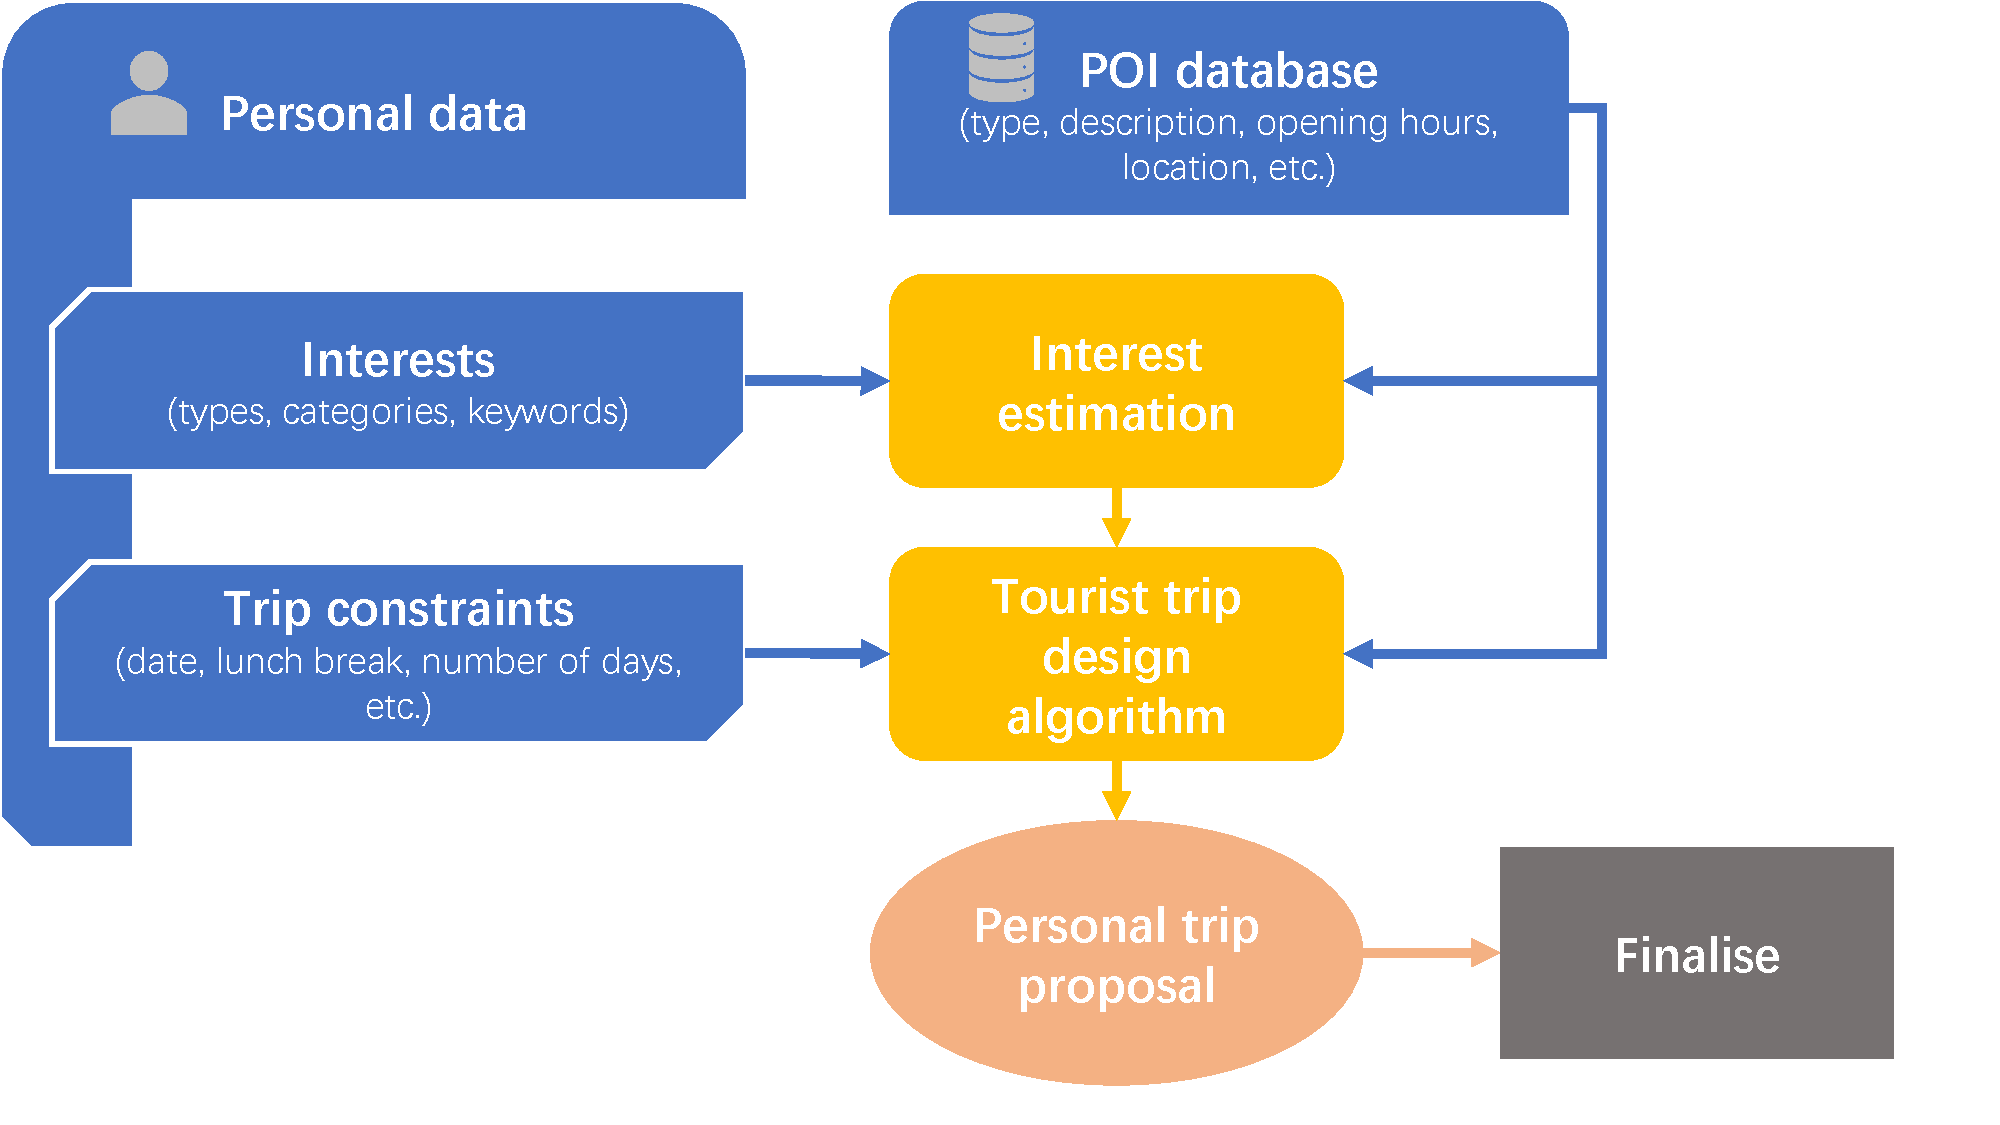
\includegraphics[width=\textwidth]{frame.pdf}
	\caption{Classical frame of tourist route recommendation.}\label{fig1}
\end{figure}

Within the proliferation of social network, people tends to share their travel experience on website, such as Flickr\footnote{https://www.flickr.com/} or Foursquare\footnote{https://foursquare.com/}, in the fomulation of photograph. According to T. Kurashima~\cite{Kurashima:2010:TRR:1871437.1871513}'s research, at least 40,000,000 geotagged photographs uploaded by 400,000 users are available in Flickr by the end of 2010. For ordinary tourists, such amount of location-based data not only give them a chance to appreciate the beauty of other cities, but also help them to discover some admired fun places or restaurants. For recommendation systems, they can figure out where a tourist went, when he went and even estimate how long he stayed in the place through analyzing the photographs taken by a user, which help recommenders to have a better knowledge of tourists' interest and provide a personalized route more in line with the taste of tourists. Extracting tourists' itineraries and futher acquire their interest through these shared photographs has been shown to be an effective method. These geo-tagged photographs taken by different users in different POIs can also reveal the popularity of POIs~\cite{lim2015personalized,memon2015travel}. 

In addtion to photographs, the dramatically increasing GPS trajectory data can also help system to do recommending jobs. Accompanied by the popularity of mobile devices, GPS trajectory data can also reflect tourists' behaviour. And compared to the discretness of photographs, users' behavior reflected by GPS trajectory data is undoubtedly more accurate. Therefore it is a wonderful idea to acquire essential information fore recommendation based on these data~\cite{7113313,Zheng:2009:MIL:1526709.1526816}. Others think of GPS trajectory data as users' browsing record and thus give a prediction of where user might go next~\cite{doi:10.1111/tgis.12248}. Whereas for most of the existing work~\cite{7113313}, such trajectory data are used only for single attraction recommendation (or a list of attractions for choosing one). Seldom do they try to use these data to commit a complete route recommendation. On the contrary, they always turns the problem into the TSP or OP problem and find ways to solve these two NP-hard problem. 

Generally speaking, the recommendation system serves as a tourist guide for the users, whereas the tourist guides in reality provide advice based on experience of other travellers while the recommendation systems provide advice based on calculations. Compared to calculations, experience-based inference is usually faster. Compared to inference, calculations tend to be more accurate. We tried to figure out a method that combines the speed of the inference and the accuracy of calculations. Hence we construct a novel model for recommending based on shared tourists' routes before in the city just as the way an experienced tourist guide works.

We figure out that tourist route the route can be treated as some POIs ordered by the visiting time, and thus can be treated a special time sequence. In past decades, machine learning has developed rapidly and has been proven to achieve good results in handling time sequence, for example in the Natural Language Processing (NLP) filed~\cite{DBLP:conf/acl/CohnHB18}. Forasmuch we handle this unique time sequence based on machine learning method. There are numerous work~\cite{Liu:2017:EEP:3115404.3115407} focusing on the single POI recommendation mentioned before. However few of them pay attention to utilize learning method to construct a realistic route for tourists. Another assumption that prompted us to think of this method is that similar users will take a similar trip in the same city. To our best knowledge, we are the first one to adopt a machine learning method to generate tourists' routes based on others' travelling trajectory data. And to futher exploit the value of all data sources, we gather the essential information from photographs taken in the POIs.

Despite the fact that idea of applying machine learning to construct a personalized route sounds appealing, there are still several challenges needed to be conquered. (i) How to formulate a reasonable route. Designing a route without limitations is quite simple. The simplest way is to arbitarily pick the next POI, which always provides a ridiculous route. (ii) How to generate a personalized route for each user. Different users might have different interest in the same POI. It is ridiculous to recommending the same route or similar routes for all the target users.

To alleviate various challenges and address the trajectory-based recommendation system, we introduces our \emph{LearningTour}  model. This model is constructed based on the encoder-decoder (or called seq2seq model)~\cite{DBLP:conf/nips/SutskeverVL14} which is widely used in NLP field. The main idea is considering the route generation process as a kind of text generation process, since the route and the text are both, to some degree, a kind of time series. This commonality enables us to recommend target users for a reasonable route conveniently and effectively. The encoder in our model is reposible for encoding the users' interest into a fixed-length context vector and the decoder takes charge of decoding the context vector back to the recommended route.

In general, our main contributions are as follows:
\begin{itemize}
	\item We originally combine the machine learning and trajectory data to generate a personalized route for tourists, not just pick up the similarest users' route for the target user.
	\item We propose a model to illustrate the combination of machine learning and trajectory data.
	\item We port the seq2seq model which is proved to be effective in NLP field to the recommendation system.
	\item We provide a novel approach to solving the OP problem.
	\item We conduct extensive experienments to verify the effectiveness of our model.
\end{itemize}

The remainder of this article is structured as follows. In Sec. 2 we dissuses the related work of tour recommendation. In Sec. 3 we set forth the formal defination of the problem. Our model is introduced in Sec. 4, and the experimental results are discussed in Sec. 5. We conclude the article in Sec. 6.

\section{Related Work}
\quad\, Tour recommendation has become a well-studied field, due to various applications\cite{8509321, 10.1007/978-3-319-91452-7_45}. In existing work, the recommendation content includes one single POI or several unrelated POIs\cite{AAAI159560}, a sequence of several related POIs\cite{doi:10.1080/13658816.2018.1458988} and next POI\cite{doi:10.1111/tgis.12248}. The generic personalised tourist route generation problem was defined as \emph{Tourist Trip Design Problem} (TTDP)\cite{Vansteenwegen2007}. This problem has produced several new variants over years. Zheng\cite{zheng2017using} put forward the consideration of the influence of season on attractions. Herzog\cite{herzog2017recommending} changes the target tourists from one person to the group. Gavalas\cite{gavalas2015ecompass} took transportation and lunch time into consideration. Herzog\cite{herzog2016exploiting} illustrates the interactions between POIs. Wang\cite{wang2018etour} considered the super poi (larger than common poi). And the data sources have also changed a lot during decades, from the questionare to the geo-tagged photographs\cite{SUN2015110} to the GPS trajectory data\cite{10.1007/978-3-319-91452-7_45, 8509321}. For an overview of the general field of tour recommedation, we refer to the survey conducted by Souffriau\cite{souffriau2010tourist} and the survey written by Gavalas\cite{gavalas2014survey}.

For those works using trajectory data to do route recommendation, which is highly related to our work: Zheng\cite{Zheng:2009:MIL:1526709.1526816} took such data as a source to generate users' behaviour. Dai\cite{7113313} mined users' interest through the data.  The only one that tried to apply machine learning method into route recommendation is Wan\cite{doi:10.1080/13658816.2018.1458988}. However he only thought of the route generation process as a classification process and thus applied KNN algorithm and Bayes classifier. Most of the route generation based on trajectory data are most used in vehicle future location prediction\cite{10.1007/978-3-319-91452-7_45}, robot navigation, or vehicle routing\cite{8509321}, while many work based on trajectory data in POI recommendation recommends only one single POI\cite{10.1007/978-3-642-35236-2_20}. Another difference between the earlier works and our work is that on the using of trajectory data, we only focus on the sequence of POIs visited by tourists instead of considering each exact timestamp when the tourists were.

With the development of machine learning, more and more people tried to adopt machine learning method in POI recommendation. It is shown that machine learning has achieved good results in POI recommendation. Sun\cite{sun2015road} showed a brilliant accuracy in calculating the popularity of route by machine learning with related parameters (i.e. the number of visited tourists). Dai\cite{7113313} adopted a Gaussian mixture model to define users' satisfaction formula. Memon\cite{memon2015travel} introduced a Probabilistic Bayesian Learning Framework to offer a personalized recommendation. Nevertheless, hardly any work pays attention to solving the route recommendation through machine learning method. Most of the work mentioned above turns the problem to the Orienteering Problem or its variance after gathering tourists' interest, POIs' attributes and constraints through tradition, non-learning method. Namely Lim\cite{lim2015personalized} adopts lpsolve to solve the problem in the form of linear programming. Baraglia\cite{10.1007/978-3-642-35236-2_20} applied a quard-tree on manage the problem.

Most of the work mentioned above regards the target city, while offering advice for a target user, as a city completely unrelated to the one when they recommend for the previous user. Forasmuch these work provide advice based on exquisite calculations, which is relatively slow than inference from experience. The method shown in Lim\cite{lim2015personalized} takes several seconds or even dozens of seconds to recommend for one user, which is intolerable for recommending for hundreds of users at this speed. The past two decades witness the rapid development of machine learning and its effectiveness based on knowledge-based inference. We recourse to machine learning method to provide an accurate and rapid way of recommendation. 

As mentioned above, we consider the route generation process as a text generation process, which has been well-studied\cite{NIPS2014_5423}. Such generation process takes a fixed-length vector (the number of categories of the POIs) as input and outputs a variable-length POI sequence. Since the seq2seq model\cite{DBLP:conf/nips/SutskeverVL14} is widely acclaimed in handling problems with different input, we adopt the design of the this model and port it to our recommendation process.

\section{Background}
\subsection{Preliminaries}
\quad\, Assuming there are $n$ POIs in the target city, let $P=\{p_1,p_2,\cdots,p_n\}$ be the set of these $n$ POIs. Each POI $p_i$ is given a label $C_{p_i}$ to represent it category (i.e. Amusement, Park, Entertainment, etc.) and use the latitude and longtitude of its center to indicate its position. We give each POI $p_i$ a score (weight) $w_i$ to illustrate how does the tourist prefer the POI $p_i$. The detail of this score function will be discussed later in Sec. 5. In addition, we define a function $T(i, j)$ which represents the time cost tourists take from the POI $p_i$ to the POI $p_j$. The value of the $T(i, j)$ is affected by the distance between the POI $p_i$ and the POI $p_j$ and the travel speed of the tourists, which depends on the mode of transportation they take and the traffic condition of the city. To simplify the problem, we unify the travel speed to \SI{10}{\kilo\meter/\minute} which we thought is a leisure walking speed and ignored the traffic condition of the city. 
\begin{definition}
	A \textbf{POI Graph} is an undirected graph $G=(V,E)$, where $V$ is the set of POIs in the city and $E\subseteq V\times V$ is an edge set. Each edge $e_{ij}$ is labeled by a cost function $T(i, j)$ and each vertice $v_i$ is labeled by a category $C_{p_i}$
\end{definition}

Hence all the POIs in the target city can be represented by a POI Graph, where $V=P=\{p_1,p_2,\cdots,p_n\}$ and $T(i, j)=\frac{dist(p_i,p_j)}{6}$. 
\begin{definition}
	A \textbf{User-based Graph} is a POI Graph where vertices are weighted by a score function $w_{iu}$.
\end{definition} 

Noted that the POI Graphs only differ from city to city, while the User-based Graphs differ from user to user. In other words, every tourist has his own User-based Graph, whereas they share the same POI Graph.
\begin{definition}
	A \textbf{Route} $R=\langle v_{i_1},v_{i_2},\cdots,v_{i_m}\rangle$ $(i_1,i_2,\cdots,i_m\in \{1,2,\cdots,n\})$ is a sequence of vertices in $V$, where $i_m=i_n$ if and only if $m=n$.
\end{definition}

Here we adopt the definition defined by K. H. Lim\cite{lim2015personalized} to demonstrate users' interest. We use the relative time tourists stayed at a POI than average to represent the favor level of tourists to the POI.
\begin{definition}
	\label{def4}
	A \textbf{Visit} of a tourist is defined as a tuple $V_p=(p, s, d)$, where $p=p_i\in P$ is a POI in the city, $s$ denotes when the tourist arrived at the POI $p$ and $d$ is the departure time of the tourist form the POI $p$.
\end{definition}
\begin{definition}
	\label{def5}
	The \textbf{Visit Duration} of a visitor in the POI $p$ is defined based on the Visit $(p, s, d)$. The duration time $VD_p=d_p-s_p$. If the tourist has never visited the POI $p$, the duration time is set to $0$.
\end{definition}
\begin{definition}
	The \textbf{Average Visit Duration} of the POI $p$ is calculated through $AVD_p=\frac{1}{n}\sum_{tourists}VD_p$. Here $n$ stands for all the tourists that have visited the POI $p$. Namely $n=\sum_{tourists}\mathbbm{1}(VD_p\neq0)$\footnote{$\mathbbm{1}(\cdot)$ is the indicator function}.
\end{definition}
\begin{definition}
	The \textbf{User Interest} for category $cat$ is defined to be $I_{C_m}=\sum_{p_i\in P}\frac{VD_p}{AVD_p}\mathbbm{1}(C_{p_i}=C_m)$, where $C_{p_i}$ is the label of the POI $p$ in the POI Graph. 
\end{definition}

In short, we only consider the tourists' interest for one category instead of for each POI. The main idea is that the more interest the tourist is in the POI, the longer time he will stay in the POI. And since we are recommending a route in the city the target user has never been before, we estimate the user's interest based on his historical travel in other cities and assume he has the same interest for the POIs belonging to the same category.
\begin{definition}
	The \textbf{Interest Vector} is the vector representing the interest of the tourist in all categories of POIs. It is defined as $IV = \langle I_{C_1},I_{C_2},\cdots,I_{C_q}\rangle$, where $I_{C_j}(j=1,2,\cdots,q)$ is the User Interest for category $C_j$.
\end{definition}

\subsection{Problem Definition}
\quad\, We now define the tour route recommendation problem as follows: Given the POI Graph $G=(V,E)$, tourist interest vector $\langle I_{C_1}, I_{C_2},\cdots, I_{C_q}\rangle$ and a start POI $p_s$ and an end POI $p_t$ designated by the target user, our goal is to recommend a route $\langle p_s,p_{i_1},\cdots,p_{i_m},p_t\rangle(m\leq\|V\|-2)$ for the tourist. One main difference between us and earlier work is that we do not need to construct a User-based Graph for each target user and calculate the route based on the User-based Graph, which greatly reduces the running time. 

\section{Recommendation Framework}
\quad\, We propose a encoder-decoder model (also known as seq2seq model) to accomplish the route generation following the design of Tianyu Liu\cite{AAAI1816599}. First we calculate each user's interest based on his or her travel history in other cities. We use a LSTM to encode the target tourist's Interest Vector to a context vector and then take the context vector as the input of a LSTM decoder to generate the route. 

The generated route $R$ contains $m$ POIs $\langle y_1,y_2,y_3,\cdots,y_m\rangle$ with POI $y_t$ at the time $t$. We formulate the route generation process as the inference over a probabilistic model. For each POI $p_t$ at the time $t$, we choose the POI with the largest probability over the chosen POI and the input parameters. In general, the $m$ POIs are chosen based on the following equation ($IV$ is the interest vector of the target user).
\begin{equation}
	\hat{y_t}=\arg\max P(\hat{y_t}\mid\hat{y_{0:t-1}},IV)
\end{equation}

And the goal of the whole inference process is to generate the sequence $\hat{y_{1:m}}$ which maximizes $P(y_{1:m}\mid IV)$. Considered the start POI $p_s$ and the end POI $p_t$ is designated by the user, we adapt the goal to generate the sequence which maximizes $P(y_{1:m}\mid p_s, p_t, IV)$. This goal is formulated as follow equation:
\begin{equation}
    \label{eqn2}
	\hat{y_{1:m}}=\arg\max_{y_{1:m}}\prod_{t=1}^{m}P(y_t\mid y_{0:t-1},p_s,p_t,IV)
\end{equation}
\subsection{Encoder}
\quad\, We propose an LSTM as the encoder. The encoder takes the input and encode it into a hidden state $h$. We take this hidden state as the context vector and tranfer it to the decoder as its initial state. According to the characteristic of RNN that takes into account the input data of each timestep, this context vector is equivalent to include all the information the input data contains, which can be regarded as the input vector in the state formulation. 

To be more specific, the architecture of the encoder is defined by the following equations:
\begin{equation}
    \label{eqn3}
	\left(
	    \begin{array}{ccc}
	        f_t\\
	        i_t\\
	        o_t\\
	        \hat{C_t}\\
	    \end{array}
	\right)
	=
	\left(
	    \begin{array}{ccc}
	    hard\: sigmoid\\
	    hard\: sigmoid\\
	    hard\: sigmoid\\
	    tanh
	    \end{array}
	\right)
	\left(
	    \begin{array}{ccc}
        W_f\\
	    W_i\\
	    W_o\\
	    W_c
	    \end{array}
	\right)
	\left[h_{t-1},x_t\right]+
	\left(
	    \begin{array}{ccc}
            b_f\\
            b_i\\
            b_o\\
            b_c
	    \end{array}
	\right)
\end{equation} 
\begin{equation}
    \label{eqn5}
	x_t \in IV\cup\{p_s\}\cup\{p_t\}
\end{equation}
\begin{equation}
    \label{eqn6}
	c_t = f_t*c_{t-1}+i_t*\hat{c_t}
\end{equation}
\begin{equation}
    \label{eqn7}
	h_t=o_t*tanh(c_t)
\end{equation}

Here we concatenate the user's interest vector and the specified start POI $p_s$ and end POI $p_t$ to a vector as the input of the encoder, i.e. $Input=\langle IV,p_s,p_t\rangle$ as shown in the Eqn.~\eqref{eqn5}, since for the same user, the different choice of the start POI $p_s$ or the end POI $p_t$ leads to a completely different route. This vector is treated as a time sequence with $\|IV\|+2$ timesteps and feed the encoder one timestep at a time. Different from the common use in NLP field, we do not embed the input vector, due to three considerations: (i) The input data is already in the mathematical form. (ii) The input data in the form of float number is hard to embed. (iii) The user's interest vector has already represented the features of the target user and thus has no need to be embeded.
\subsection{Decoder}
\quad\, For the decoder, we propose a dense layer after a normal LSTM. The architecture of this normal LSTM is the same as the one in the encoder. The dense layer uses a softmax function to convert the output of the normal LSTM at each timestep to the generated POI at the timestep. Following equation 1, this generated POI is predicted on the basis of all the previous chosen POIs and the context vector transfered from the encoder. Such process is fomulated as follow equations:
\begin{equation}
	P(y_t\mid H_t,y_{<t})=softmax(W_s*g_t)
\end{equation}
\begin{equation}
	g_t=tanh(W_t*s_t)
\end{equation}
\begin{equation}
	s_t=LSTM(y_{t-1},s_{t-1})
\end{equation}

where $H_t=[h_t,c_t]$ represents the encoded information of the input data ($h_t$ and $c_t$ are the last hidden state of the encoder, defined by Eqn.~\eqref{eqn6} and Eqn.~\eqref{eqn7}) and $s_t$ is the $t-th$ hidden state calculated by the normal LSTM cell. The computational details can be refered to the Eqn.~\eqref{eqn3}, Eqn.~\eqref{eqn6}, and Eqn.~\eqref{eqn7}. The whole frame of our model is shown in Fig.~\ref{fig2}.
\subsection{Training}
\quad\, In our model, we choose the categorical cross-entropy as the loss function, i.e. $L_i=-\sum y_i\log\hat{y_i}$, where $y_i$ stands for the target POI and $\hat{y_i}$ stands for the predicted POI. Actually in the dense layer, the route generated task has been partially converted to a multi classfication task. And as mentioned above in Eqn.~\eqref{eqn2}, we hope to maximize the probability that the model predict the route exactly the same as the target route. Based on these considerations, we choose categorical cross-entropy as the loss function.  
\begin{figure}
	\centering
	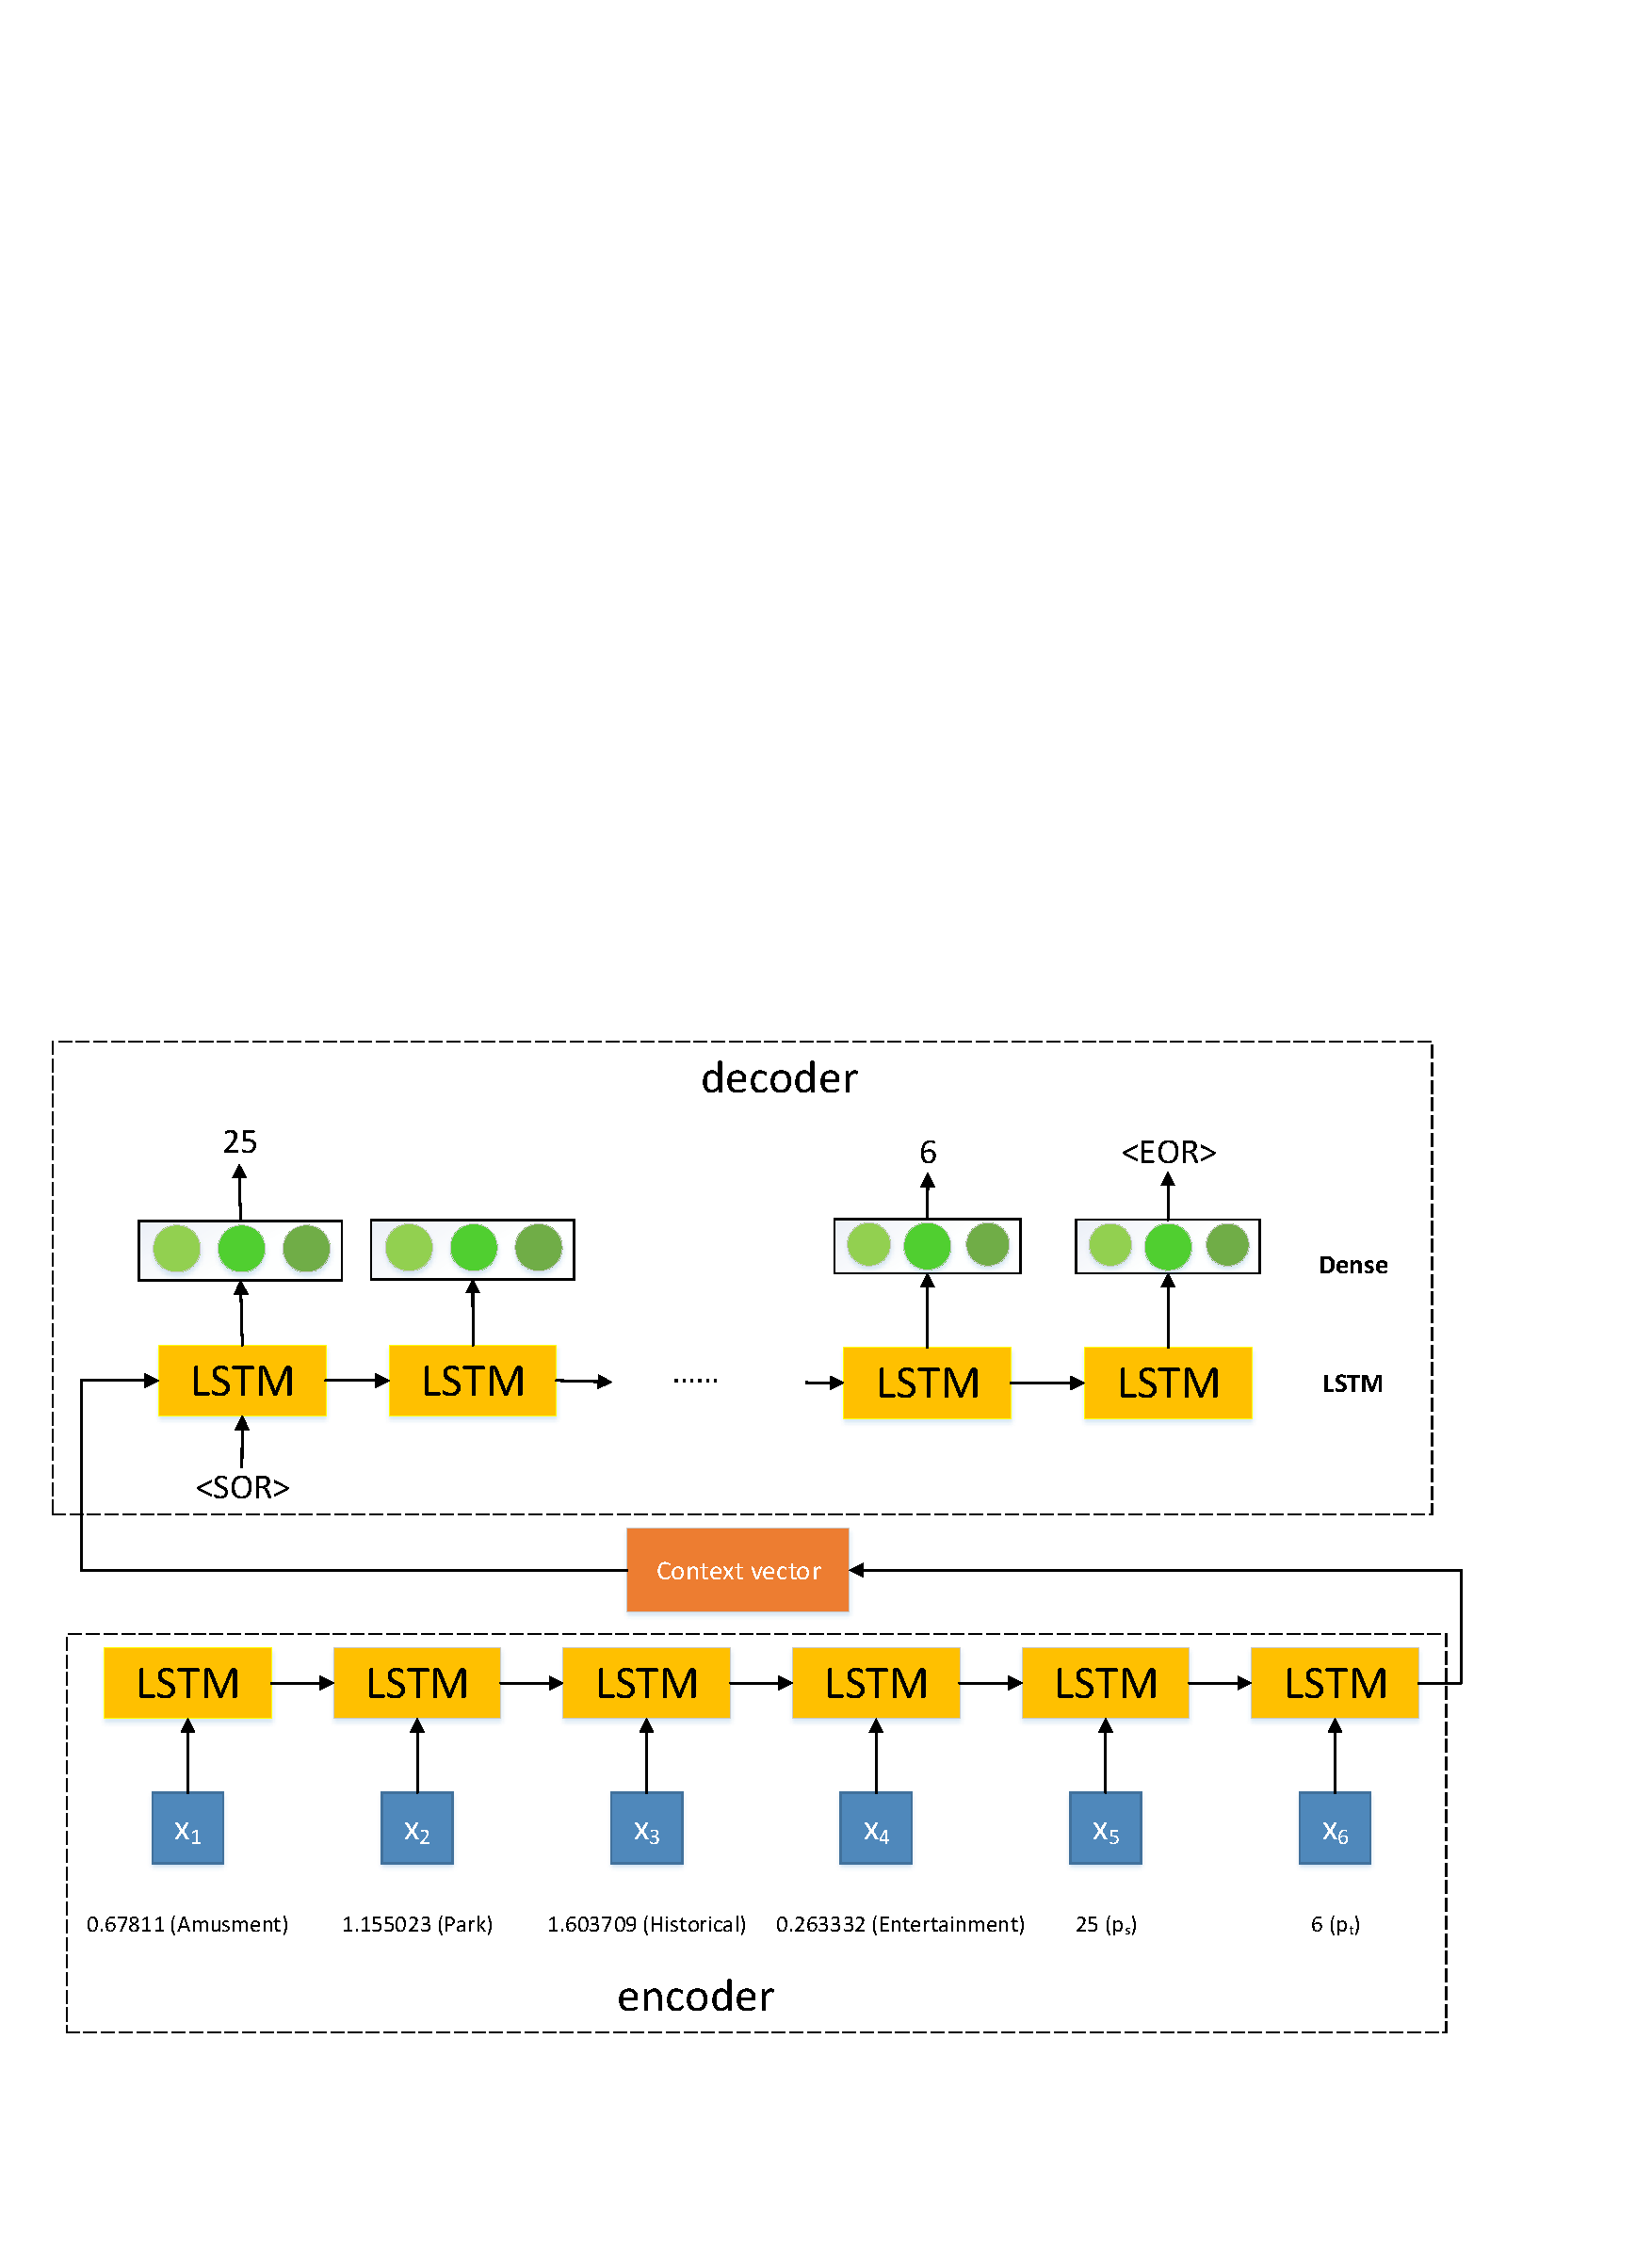
\includegraphics[width=0.9\textwidth]{model.pdf}
	\caption{The whole follow chart of how the model works to recommend a route for a tourist with interest vector $\langle Amusement,Park,Historical,Entertainment\rangle=\langle 0.67811,1.155023,1.603709,0.263332\rangle$ who specify the recommended starting from the POI with id $25$ and ending at the POI with id $6$. }\label{fig2}
\end{figure}
\section{Experiment}
\quad\, In this section, we will describe the detailed experimental settings and analysis the results. We first introduce the datasets, the baseline algorithms and the method to assess in turn. After that we will discuss the result of our experiments. 

The experiments are tested on a Intel Core i7 server with 2.60 GHz processor and 8 GB RAM. The programs are coded in Python. 
\subsection{Datasets}
\quad\, In our experiments, we use the dataset provided by K. Lim~\cite{lim2015personalized}, which is extracted from 100M Flickr photos and videos. The dataset comprises the attributes of POIs (POIs' location, POIs' category and POIs' name or ID) and users' historical travel experience in the formulation of photos. Each photo is labeled with six attributes: photoID, userID, dateTaken, poiID, poiTheme, and poiFreq. We futher cluster the photos to Visits (Def.~\ref{def4}) by taking the time the first photo taken by the user as the arrival time and the time the last photo taken as the departure time and then extract users' interest on the basis of these Visits. To ensure the best accuracy and generalizability of our approach, we only consider the travel sequence with $\geq3$ POI Visits. The detailed description of the dataset is shown in Tab.~\ref{tab1} and the saptial structure of POIs in the datasets is shown in Fig.~\ref{fig:e3}.
\begin{table}
	\caption{Dataset description}\label{tab1}
	\begin{tabular}{|l|l|l|l|l|l|}
		\hline
		City & No.of Photos & No.of users & No.of POI Visits & No.of Travel Sequences & No.of POIs\\
		\hline
		Toronto & 157,505 & 1,395 & 39,419 & 6,057 & 30\\
		\hline
		Osaka & 392,420 & 450 & 7,747 & 1,115 & 29\\
		\hline
	\end{tabular}
\end{table}

\begin{figure}
	\centering
	\subfigure[Toronto]{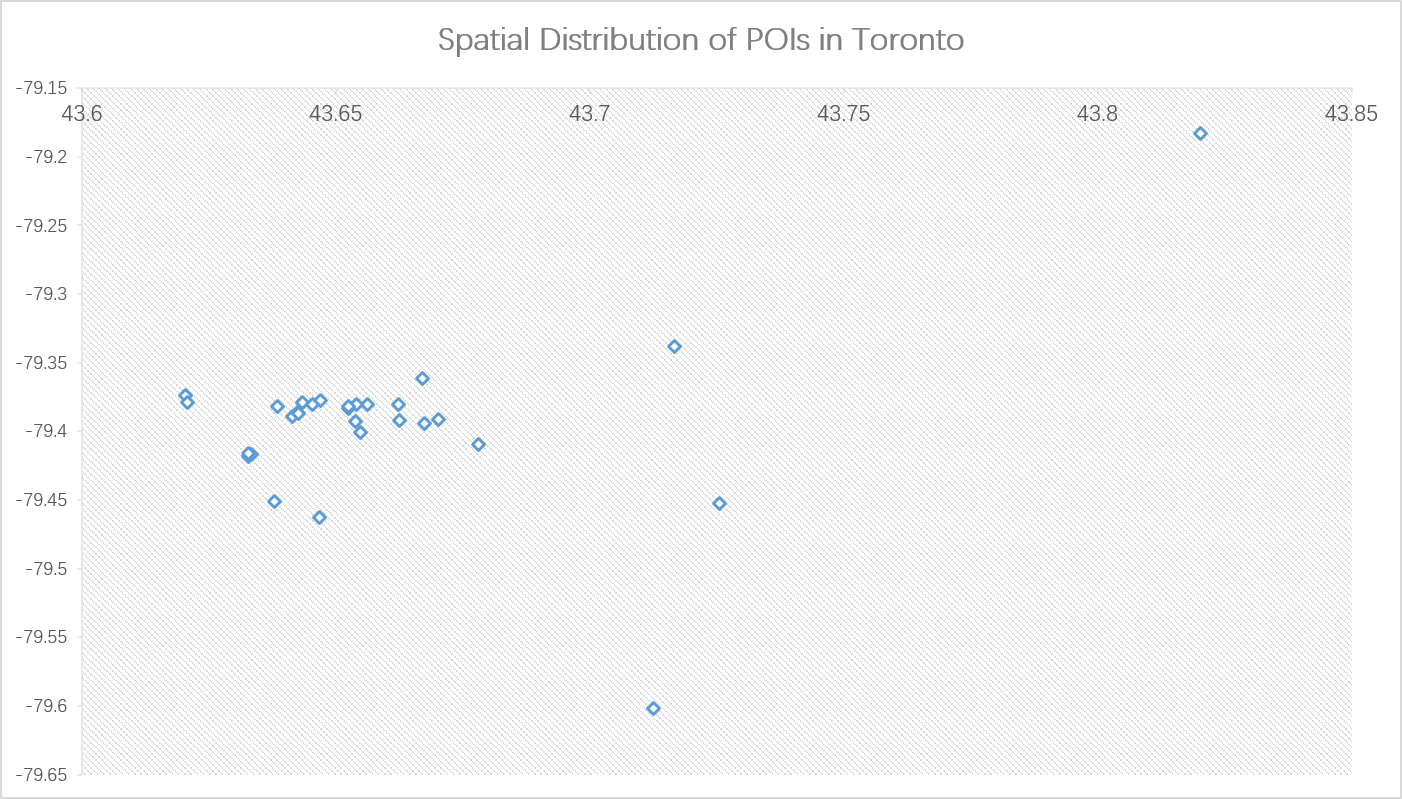
\includegraphics[width=0.48\textwidth]{Toronto.jpg}}
	\quad
	\subfigure[Osaka]{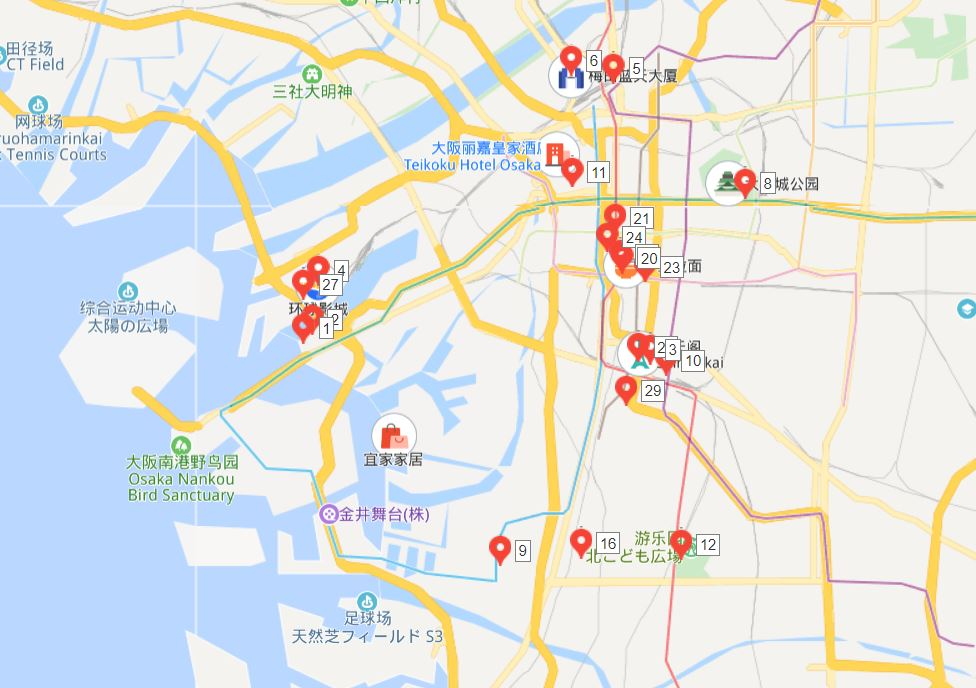
\includegraphics[width=0.48\textwidth]{Osaka.jpg}}
	\caption{The spatial distribution of POIs in the datasets. The number besides each location represents the POI's id.}
	\label{fig:e3}
\end{figure}
\subsection{Baseline algorithm}
\quad\, We choose random selection algorithm and GNU Linear Programming Kit (GLPK)~\footnote{https://www.gnu.org/software/glpk} as our baseline algorithms. Same as our LearningTour model, the random selection alogorithm commence from a given start POI $p_s$ and then iteratively choose the next POI until (i) the time budget B is not sufficient, or (ii) The chosen next POI is the given end POI $p_t$. Hence the target user's itinerary has been recommended based on the sequence the POI was chose. The GLPK method commences from a basic feasible solution, and then iteratively search for a better solution until either (i) no better solution can be found; or (ii) the best solution is proved to not exist. These baseline algorithms are explained in details as follows:
\begin{itemize}
	\item \textbf{RandomSelection:} The random selection algorithm chooses the next POI by randomly selecting from all the unvisited POIs.
	\item\textbf{GLPK:} The way to find the better solution is basically the same as the simplex method, whereas it calculates the inverse of the new matrix based on the inverse of the old matrix instead of adopting a gaussian elimination method in the successive iterations.
\end{itemize} 
\subsection{Evaluation Method}
\quad\, We evaluate our model and the other two baslines based on two aspects: the score the user get and the CPU running time it takes to provide the recommended route. We consider the score based on three aspects: users' interest in the POI, POI's own popularity, and POI's public reputation among tourists. We quantify the reputation on the basis of information crawled from TripAdvisor\footnote{https://www.tripadvisor.cn/}. The information contains the POIs' score out of 5, number of reviews, and the rank of POIs among the same category of attractions.
\begin{definition}
	The \textbf{Popularity} of the POI $p$ is calculated by $Pop(p)=\frac{visit(p)}{\max_{P}visit(p_i)}$, where $visit(p)$ represents the number of tourists visited the POI.
\end{definition}
\begin{definition}
	The \textbf{Score} of the POI $p$ is based on the Popularity of $p$ and users' reviews. 
	\begin{equation}
	S(p)=\alpha\cdot Pop(p)+\beta\cdot\frac{g}{5}+\gamma\cdot(1-\frac{1}{\#reviews})+\delta\cdot(1-\frac{rank}{N})
	\end{equation}
	
	where $\alpha,\beta,\gamma,\delta$ are all set by users ($\alpha+\beta+\gamma+\delta=1$), $g$ is average score (score of 5) graded by all the tourists who have visited the POI, $rank$ is the POI's rank among the POIs with the same category as $p$, and $N$ represents the number of these POIs.
\end{definition}

This is the same as the reality: The more popular the POI is and the higer reputation the POI enjoys, the higher score it will get.
\begin{definition}
	The \textbf{Weight} of a POI $p$ is endowed under the consideration of both the score $S(p)$ of the POI and the target user's interest in it. $w(p)=\eta\cdot S(p)+(1-\eta)I_{C_p}$
\end{definition}

$\eta$ is a weight coeffecient set by the recommendation system, depending on whether the system values users' interest more or the popularity and the reputation of a POI more.  
\begin{definition}
	The \textbf{Score} of a route $R=\langle y_1,y_2,\cdots,y_m\rangle$ is defined as the sum of the weight of each POI in the route. $S(R)=\sum_{i=1}^{m}w(y_i)$
\end{definition}

To strike a balance between the popularity of the POIs and users' interest among these POIs, we choose $\eta=0.5$ in our experiments. Noticed that for each POI $p$, we have $\frac{1}{\#reviews},\frac{rank}{N}\in(0,1]$ and $\frac{g}{5},Pop(p)\in[0,1]$. In addtion we require the weight defined by users for the aspects satisfy $\alpha+\beta+\gamma+\delta=1$, thus having $S(P)\in[0,1]$. For users' interest, which is defined through Visit Duration (Def.~\ref{def5}), we infer from common knowledge that it is a float number normally not greater than 1.5. Therefore $\eta=0.5$ will not lead the recommendation system pays more emphasis on any side. 
\subsection{Experiment Setups}
\quad\, While generating the recommended route, we add a $\langle SOR\rangle$ label at the beginning of the route and a $\langle EOR\rangle$ label at the end of the route, following the design of I. Sutskever\cite{DBLP:conf/nips/SutskeverVL14}. In other word, we adapt the route $\langle y_1,y_2,\cdots,y_m\rangle$ to $\langle SOR,y_1,y_2,y_3,\cdots,y_m,EOR\rangle$. We also take one-hot code for each POI to have a better learning effect. Other detail of our model parameters is listed in Tab.~\ref{tab:2}.
\begin{table}
	\caption{Parmeters setting for our experiments}
	\centering
	\begin{tabular}{|l|l|l|l|l|}
		\hline
		Hidden size & Batch size & Epochs & Learning rate & Optimizer\\
		\hline
		100 & 64 & 100 & 0.001 & rmsprop\\
		\hline
	\end{tabular}
    \label{tab:2}
\end{table}
\subsection{Results and Discussions}
\quad\, Fig.~\ref{fig:5} shows that our method provides a better route for tourists than the two other baselines. Despite the fact that different tourists may have different reachable maximum profits, our method outperforms the baseline methods on the whole. This fact shows that routes recommended based on other tourists' historical travel experience is more appealing than routes recommended only based on the POIs' introductions and spatial structure. We believe that the model `learns' the spatial structure of the POIs in the city from other users' experience and do the job based on what it have `learned', while each time the GLPK method provides recommendation as if facing a completely unfamiliar city and a completely unfamiliar target user. Such unfamiliar is shown to be not only a huge time overhead but also a lag behind in effect. 

\begin{figure}[htbp]
	\centering
	\subfigure[Toronto]{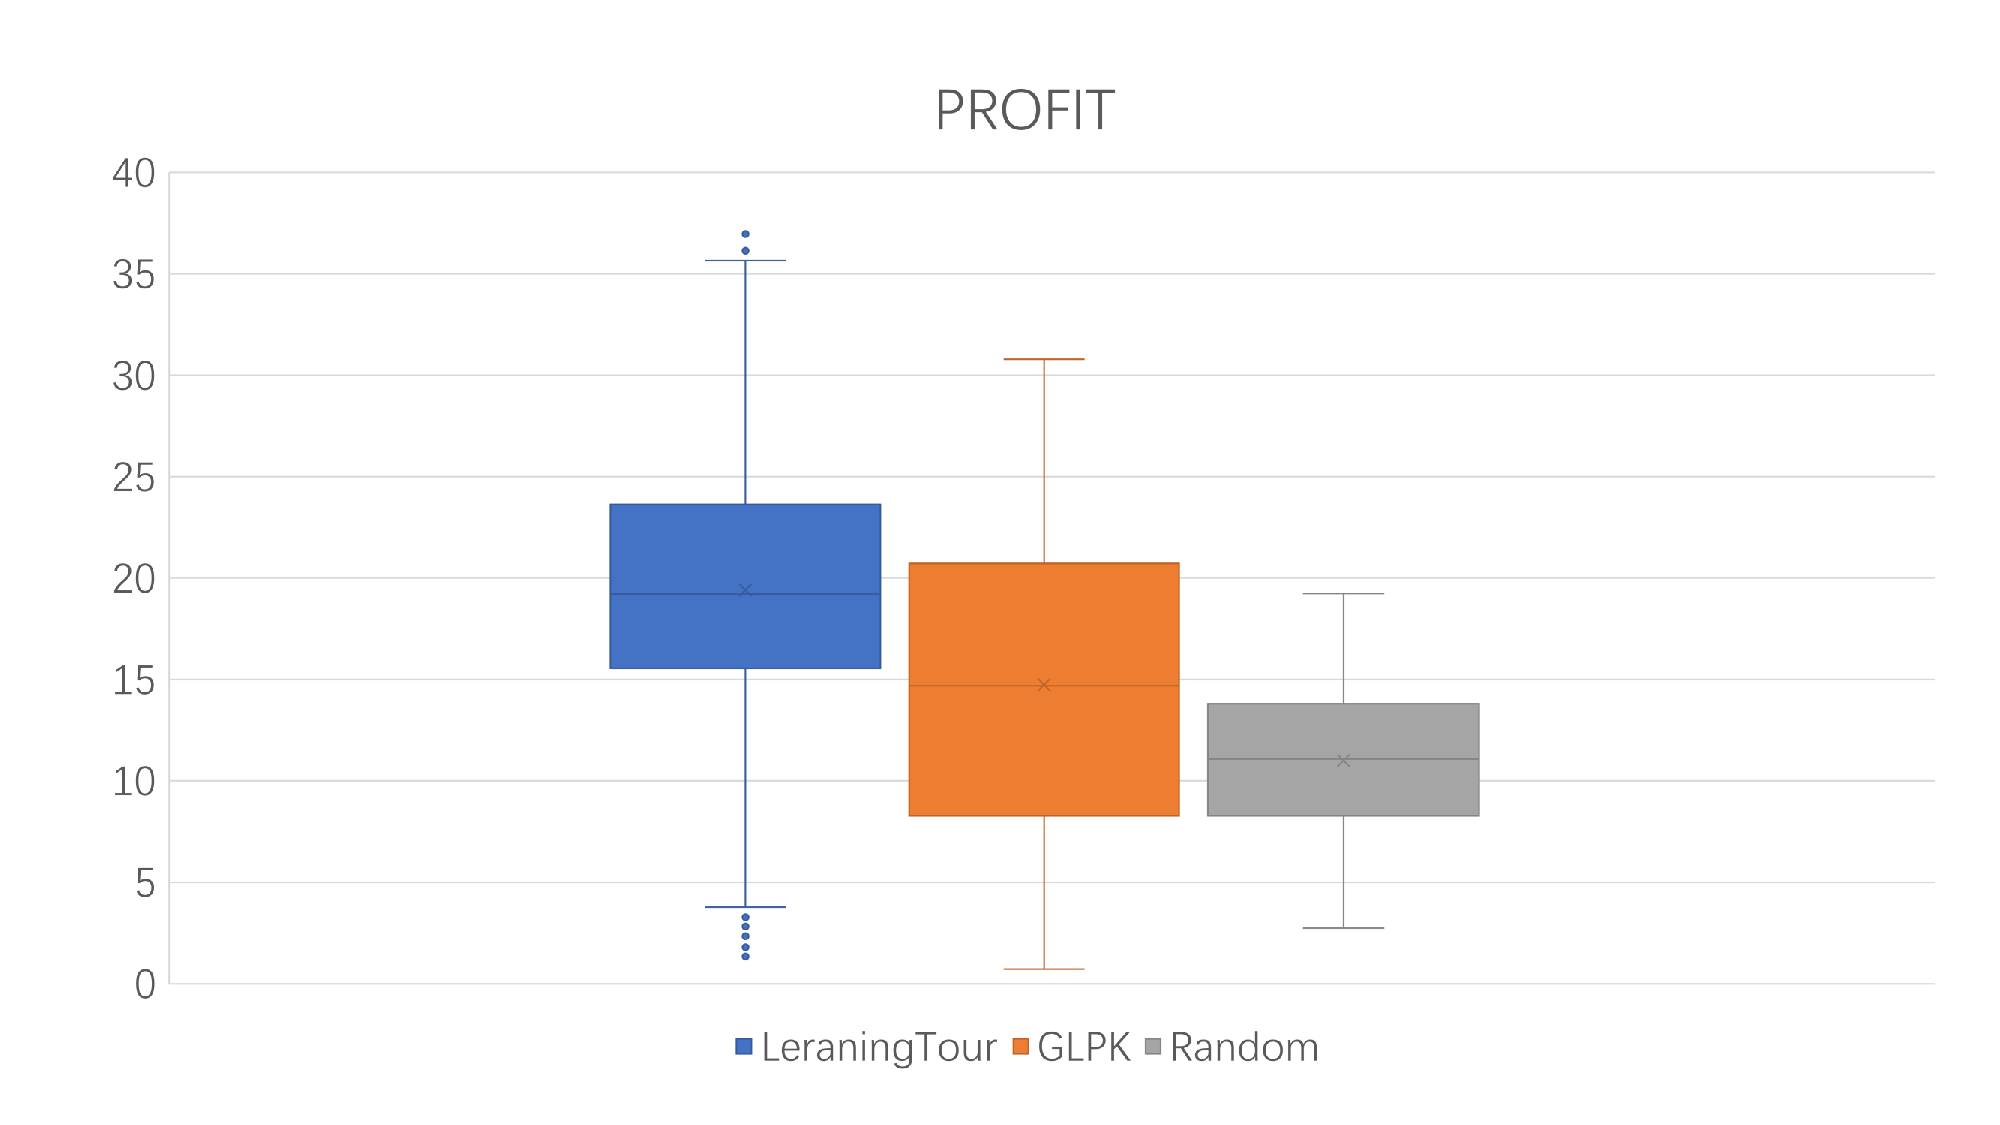
\includegraphics[width=0.48\textwidth]{TProfit.pdf}}
	\quad
	\subfigure[Osaka]{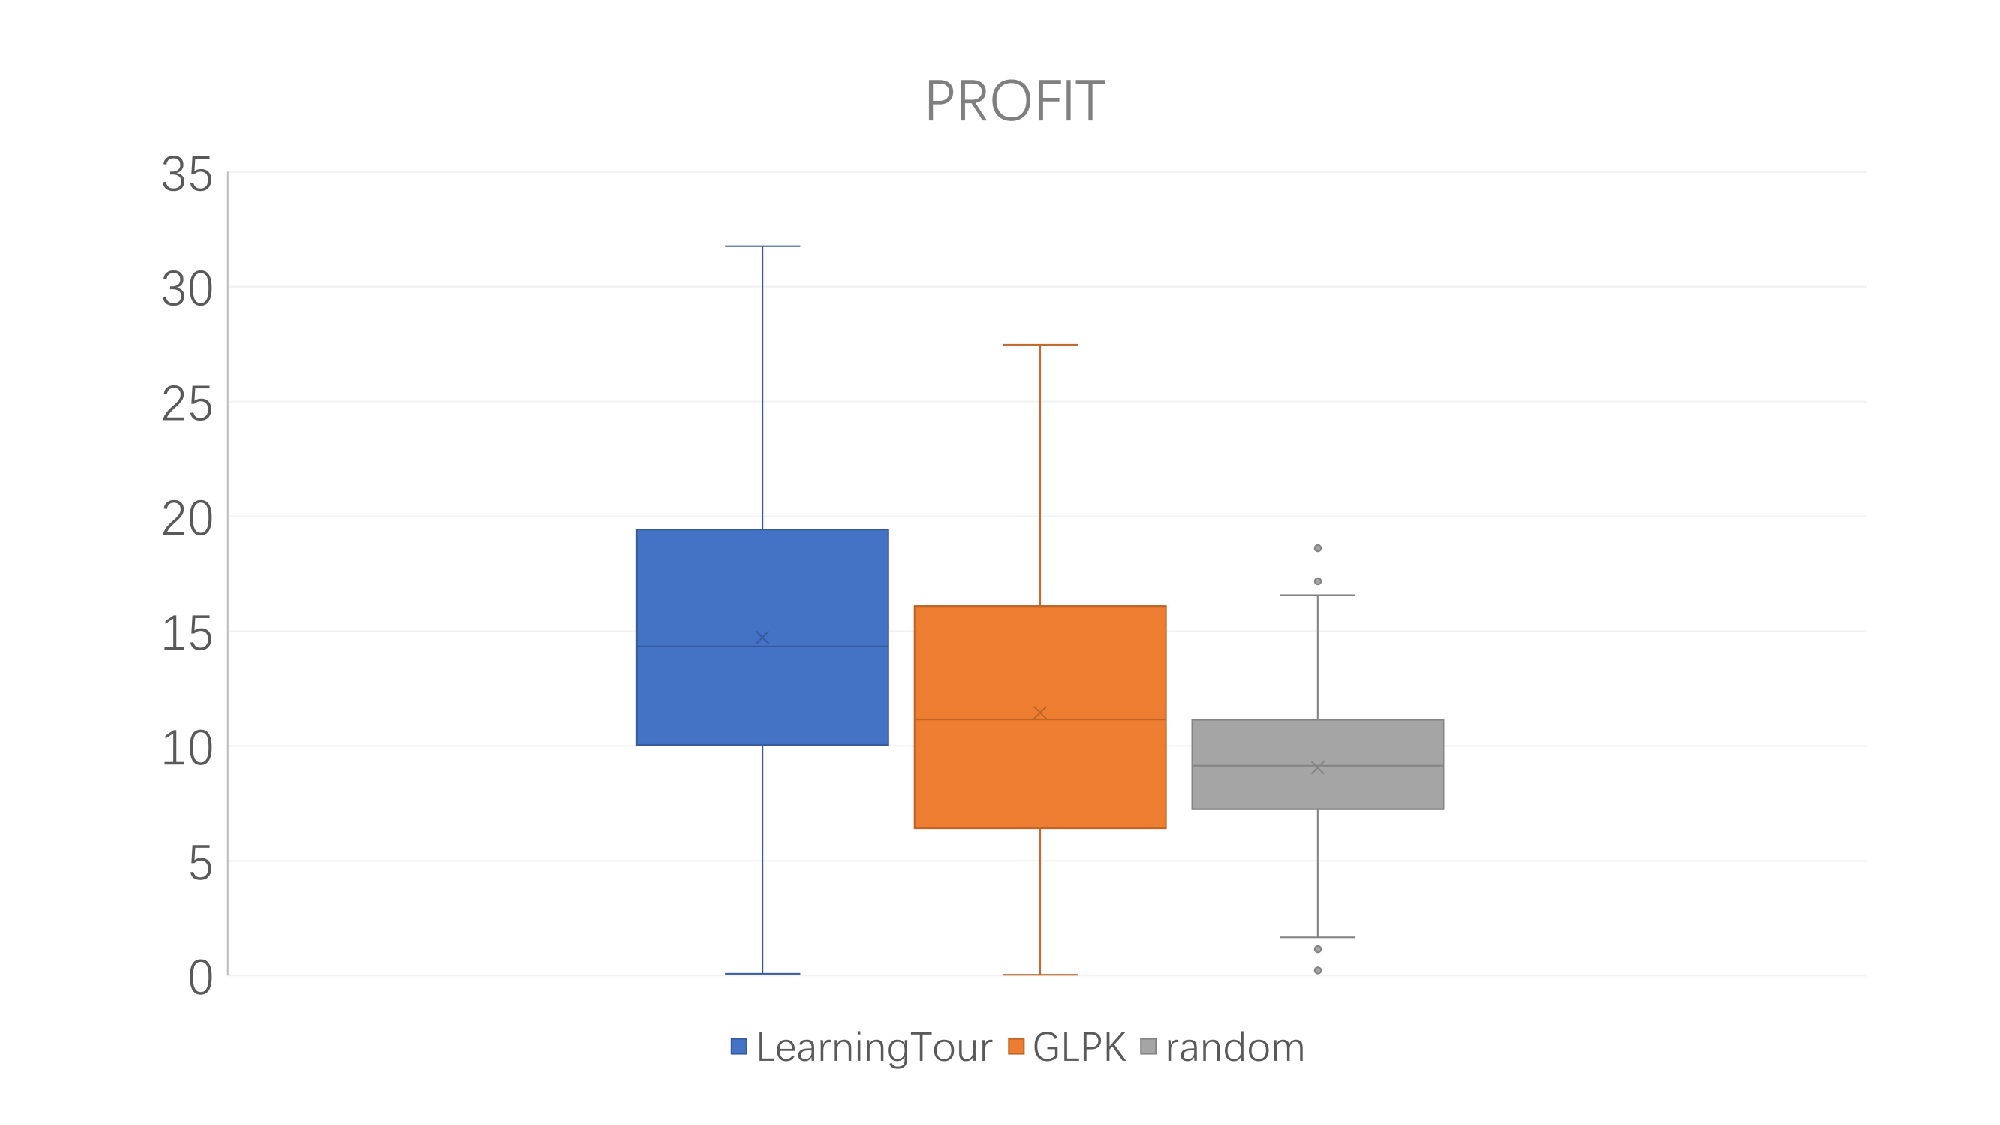
\includegraphics[width=0.48\textwidth]{OProfit.pdf}}
	\caption{Profits of different solutions on two datasets}
	\label{fig:5}
\end{figure}

As shown in the Fig.~\ref{fig:4} and the Fig.~\ref{fig:3}, our model is one to two orders of magnitude faster than the GLPK method. In addition, shown in Fig.~\ref{fig:3}, the GLPK method presents a big difference of running time on different datasets, while our model takes similar time to recommend regardless of the difference in the topology of the POIs of different cities. Moreover even for the same dataset, the running time of the GLPK method ranges a lot (from about 0.3 seconds to almost 20 seconds) as shown in Fig.~\ref{fig:7}.  
\begin{figure}[htbp]
	\centering
	\subfigure[Toronto]{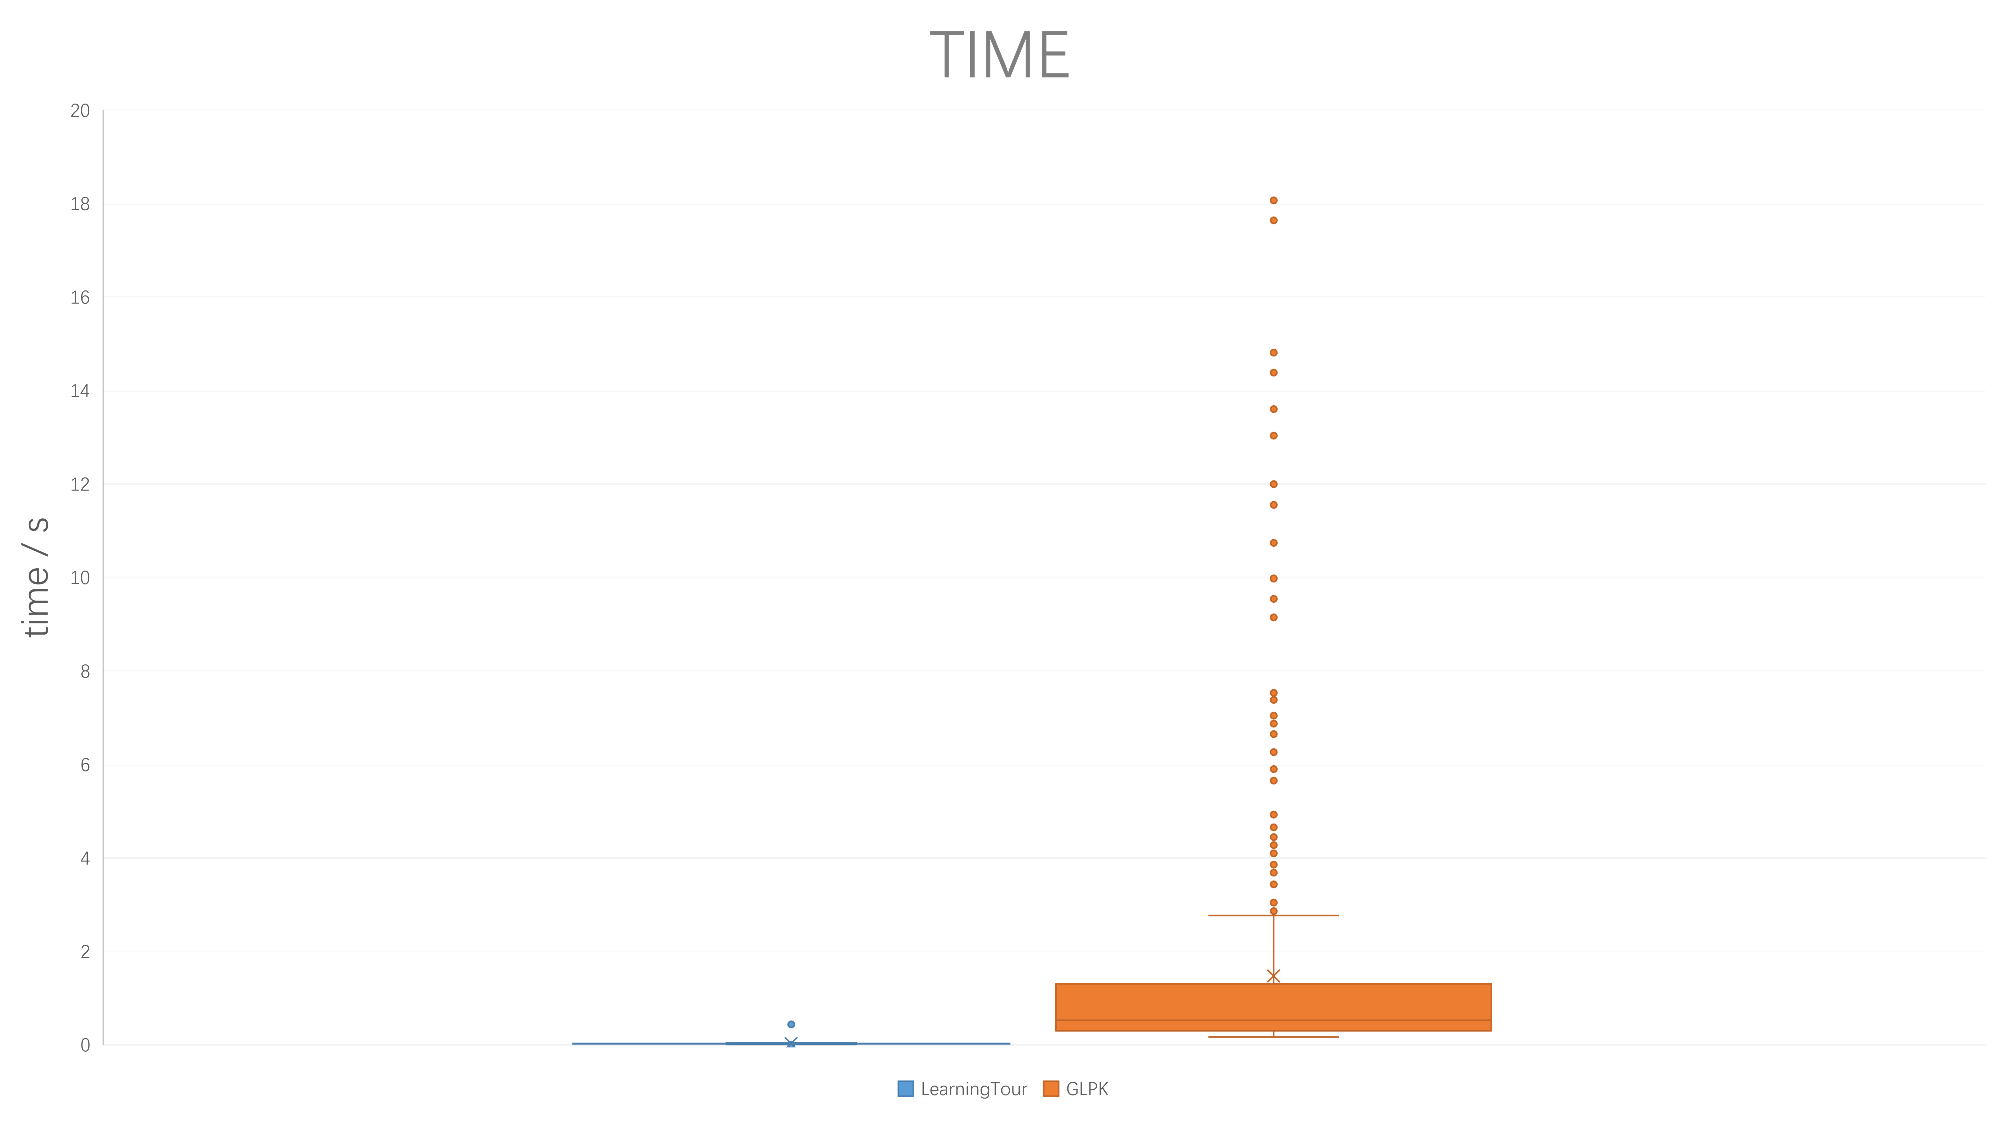
\includegraphics[width=0.48\textwidth]{tmp.pdf}}
	\quad
	\subfigure[Osaka]{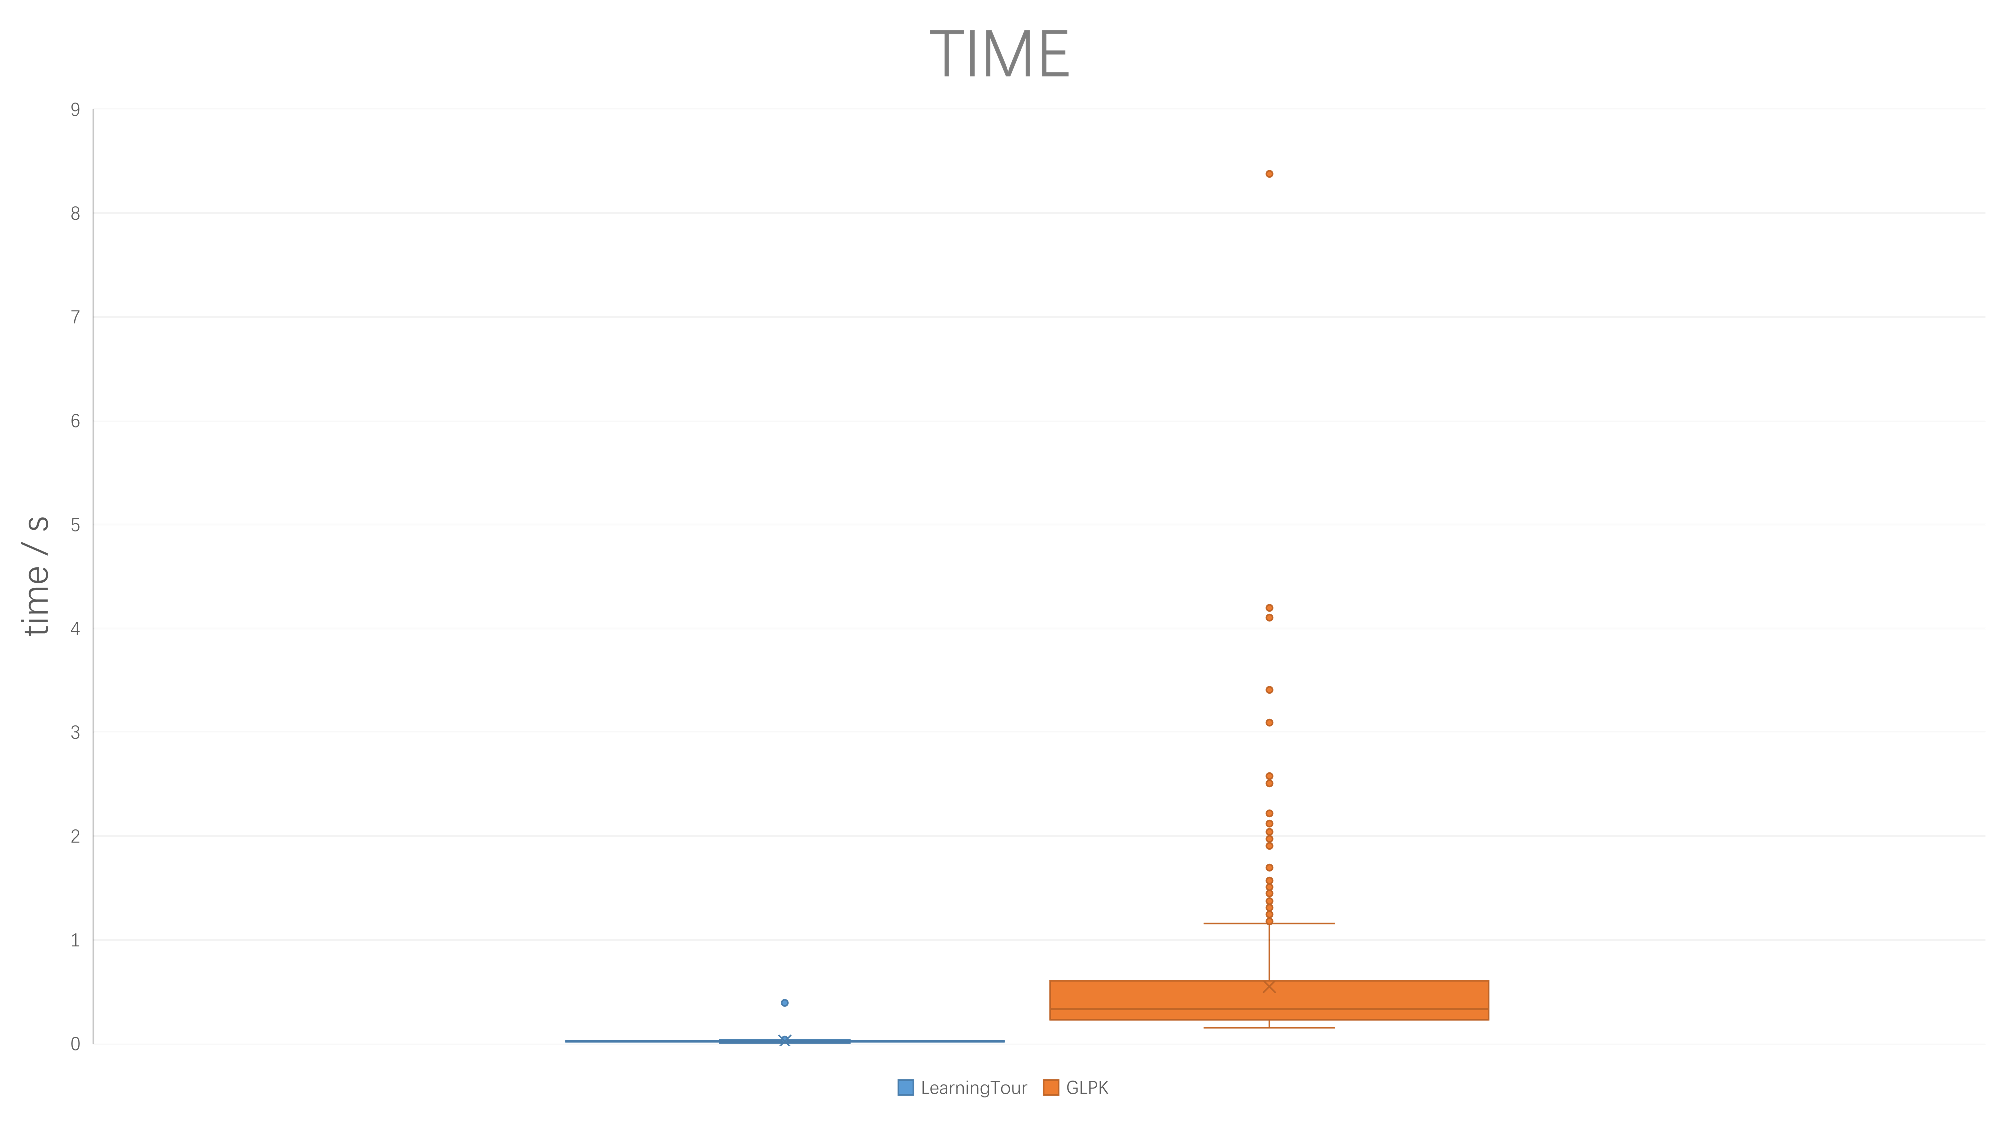
\includegraphics[width=0.48\textwidth]{Otmp.pdf}}
	\caption{The CPU Time of different solutions on two datasets}
	\label{fig:7}
\end{figure}
\begin{figure}[htbp]
	\centering
	\subfigure[Toronto]{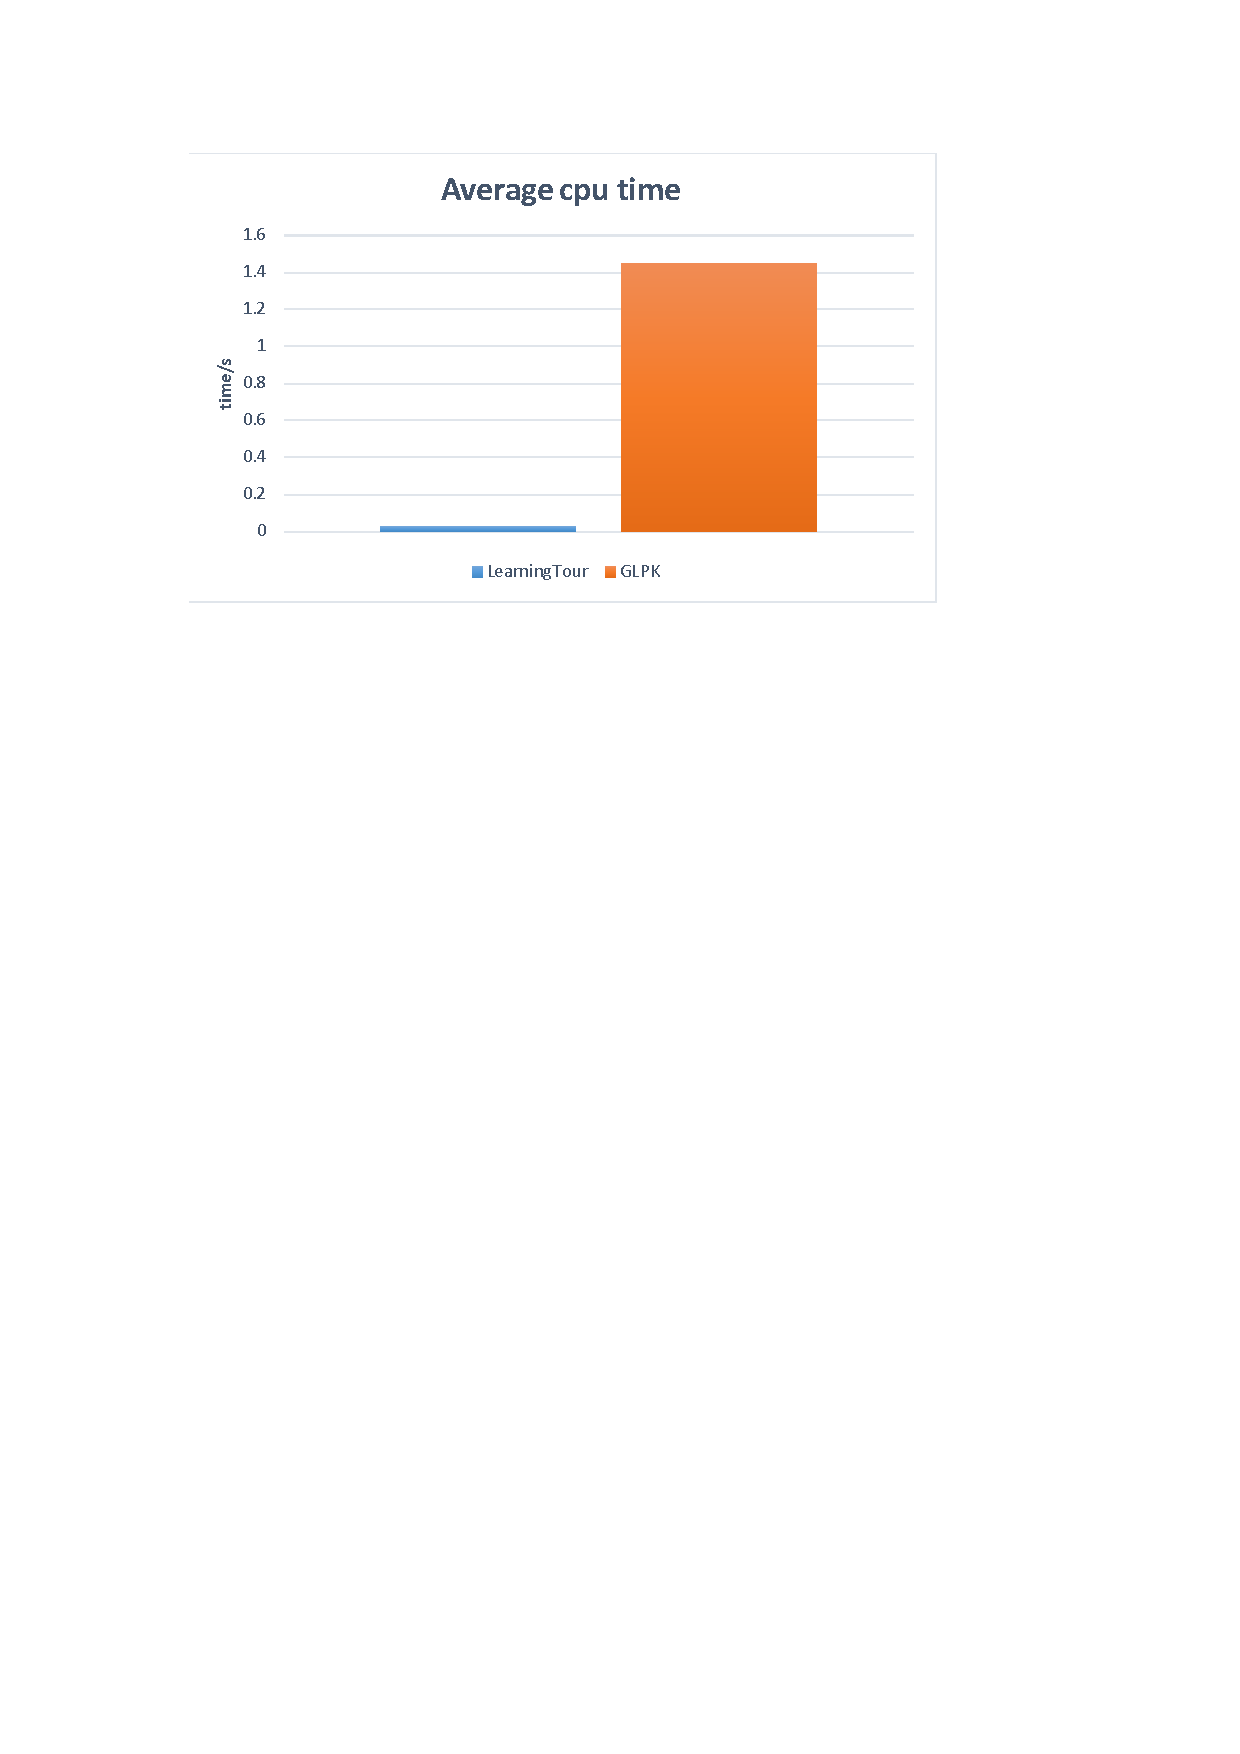
\includegraphics[width=0.48\textwidth]{AVT.pdf}}
	\quad
	\subfigure[Osaka]{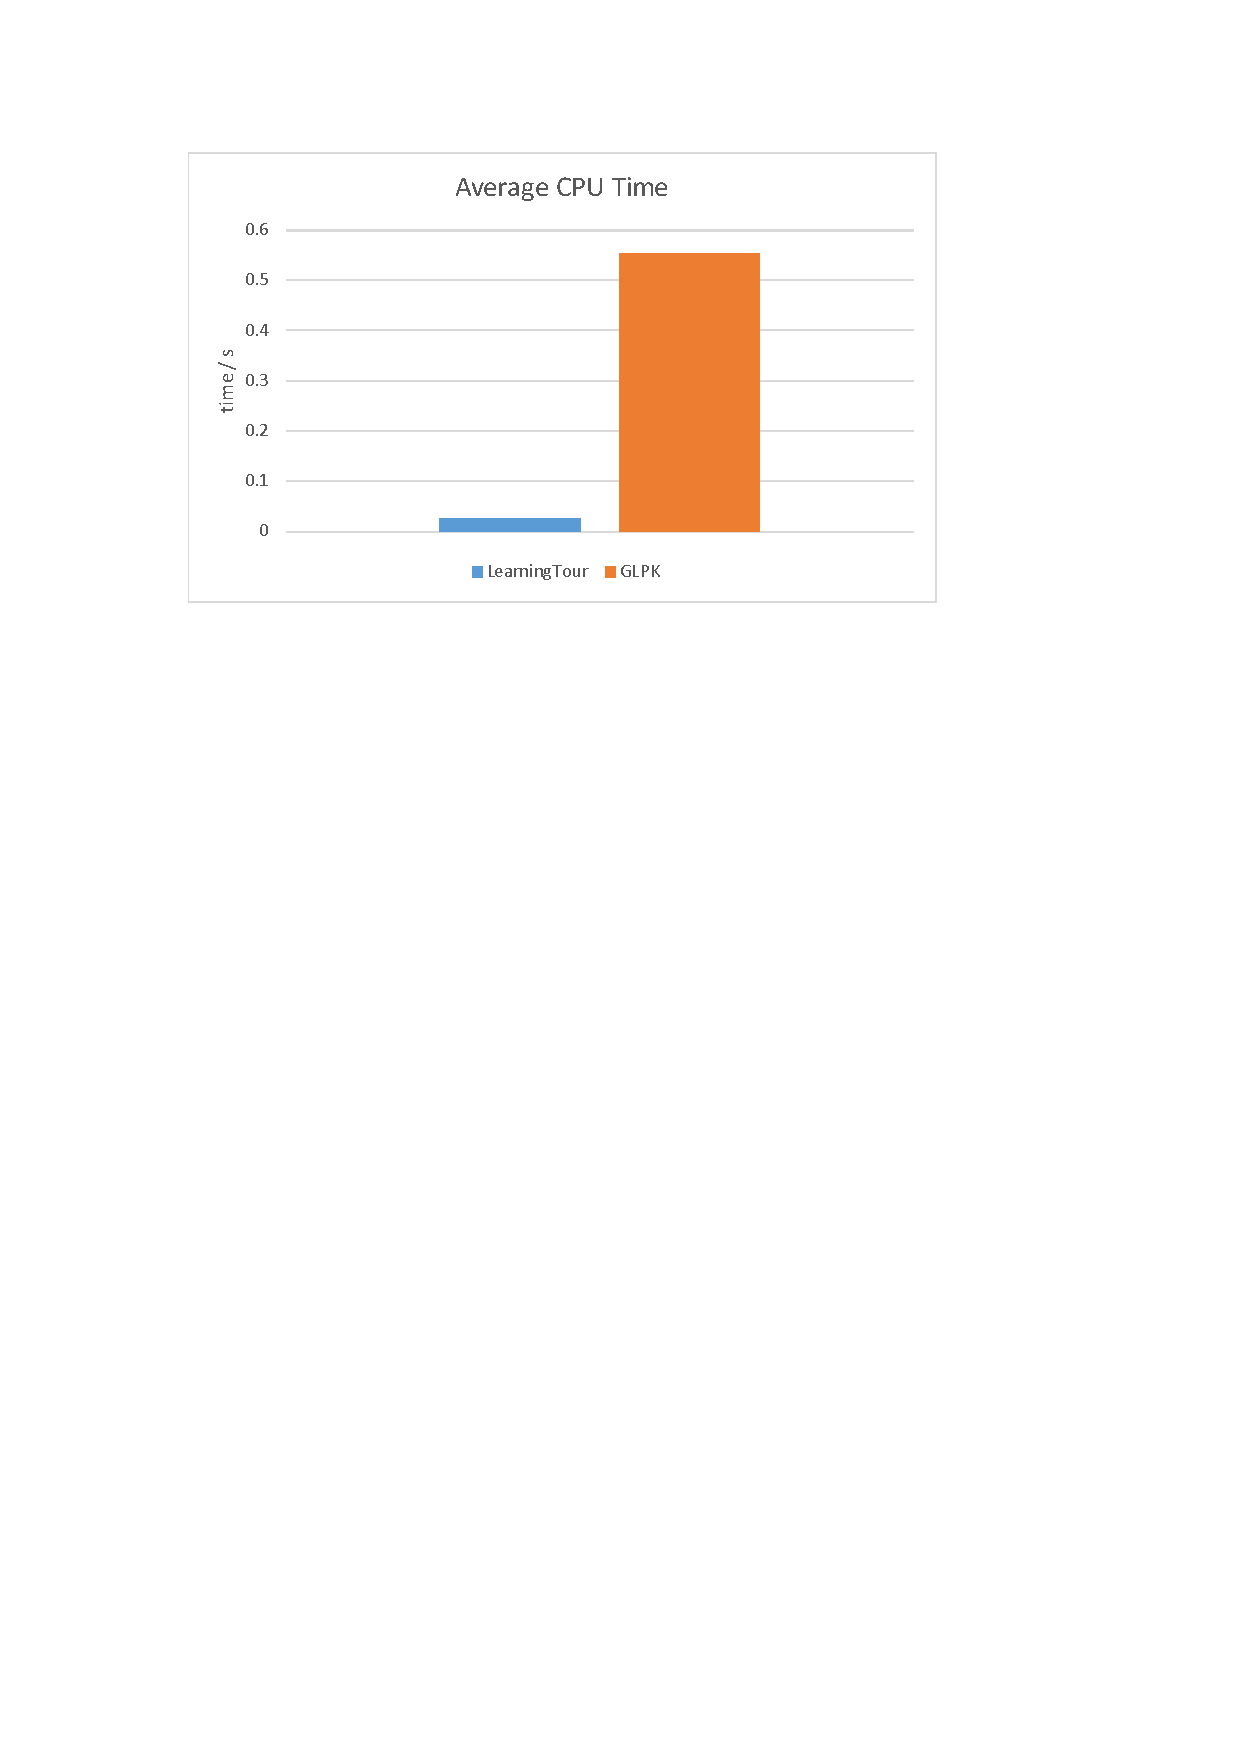
\includegraphics[width=0.48\textwidth]{AVTO.pdf}}
	\caption{Average CPU Time of different solutions on two datasets}
	\label{fig:3}%
\end{figure}

The reason that our model runs far more faster and more steady than the GLPK method is due to it skipping the process of constructing the unique User-based Graph for each user. Our model simplify the three-step process (acquire users' interest, scoring each POI based on users' interest, and then do the recommending job based on the scored graph) in a two-step process (acquire users' interest and then do the recommendation job). Another reason is that the geographical structure of the POIs in the city does not participate in the recommendation during the whole process at all. The computation of this complete graph (usually contains 30 or even more vertices) can be a huge overhead.

Futhermore we found that our model is more robust compared to the GLPK method. In both datasets we found there exists some POIs that have no records about the previous visited users. In the GLPK method, it takes a far longer time than usual when it needs to calculate through these POIs (shown in Fig.~\ref{fig:7}) while in our approach such obstacle does not exist. Our model presents a steady running time facing the deficiency of the data, for it `learns' to avoid the POI at once when meeting with it without calculations, which is another advantage of inference based on experience over calculations. 
\begin{figure}[htbp]
	\centering
	\subfigure[Toronto]{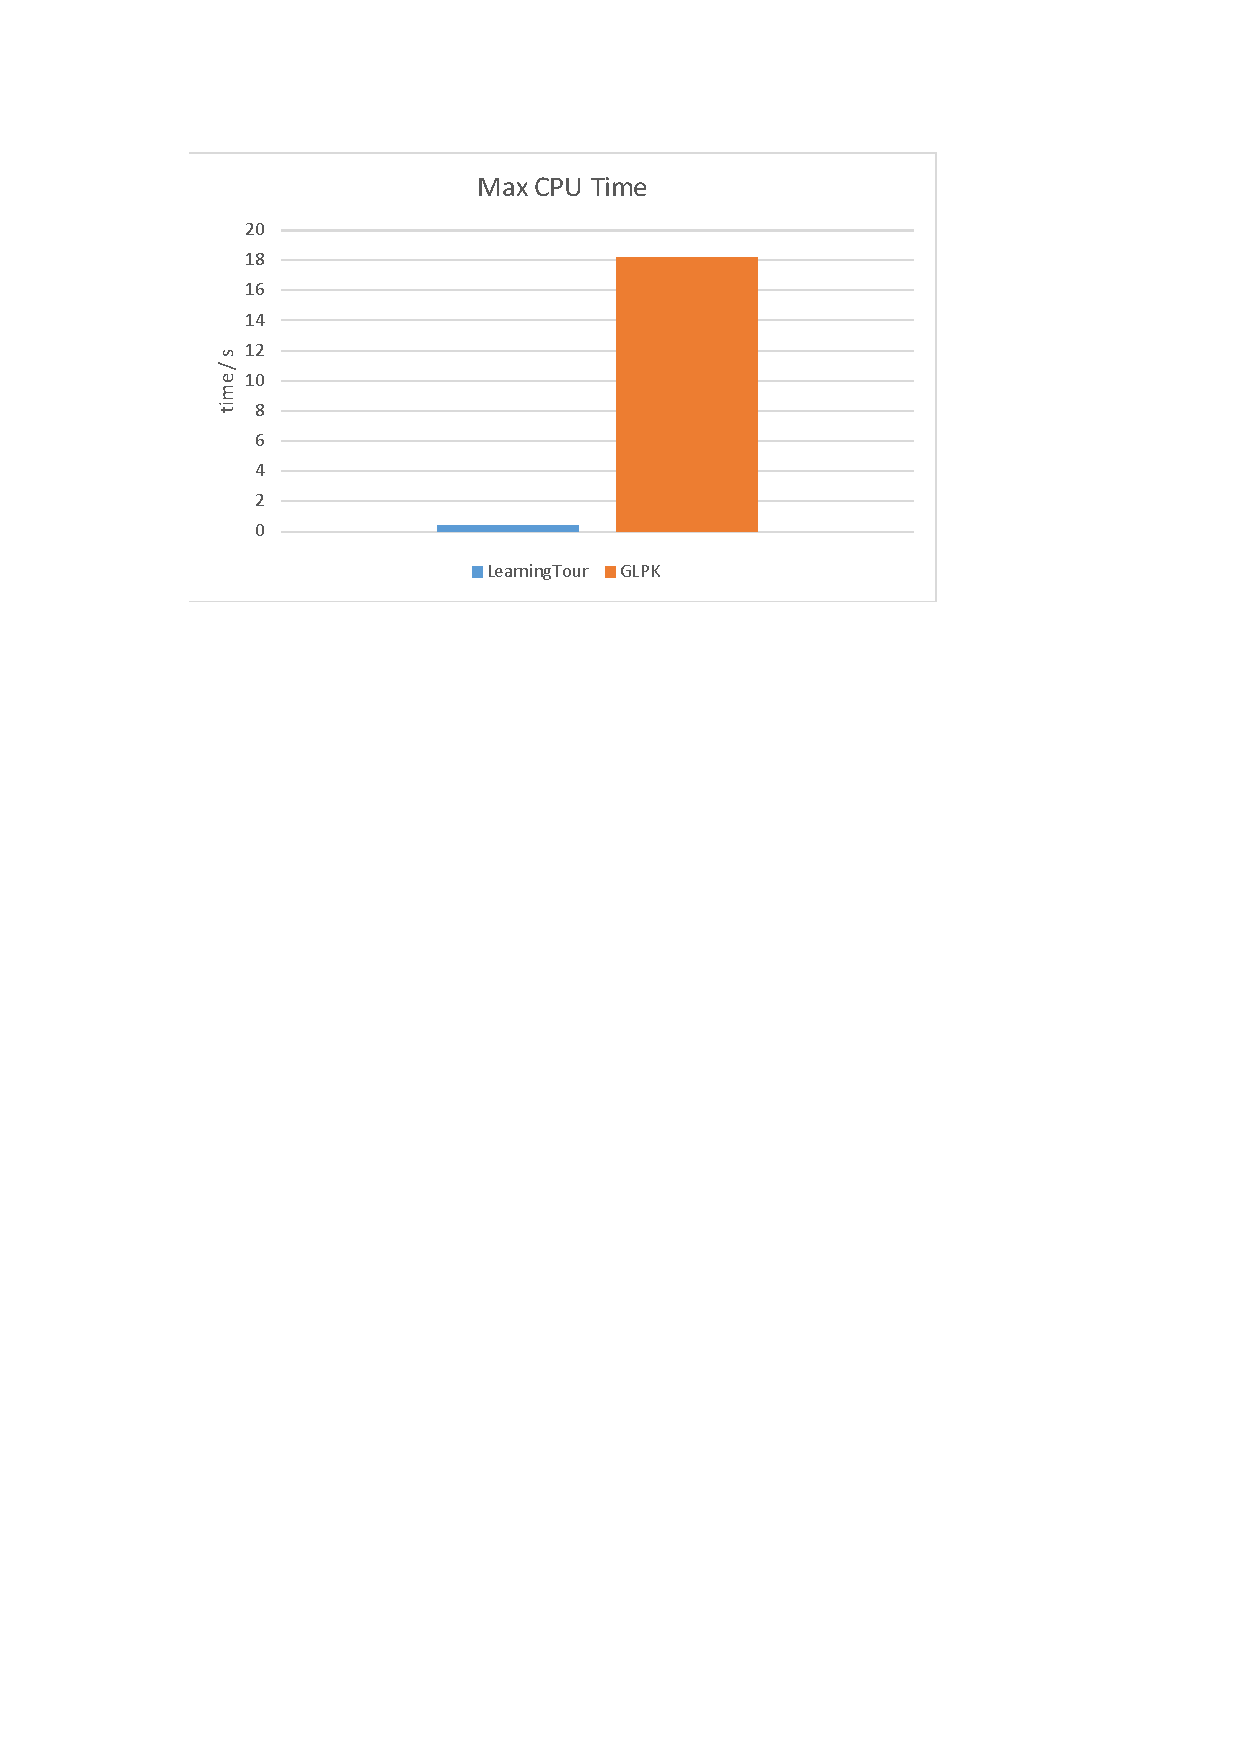
\includegraphics[width=0.48\textwidth]{MT.pdf}}
	\quad
	\subfigure[Osaka]{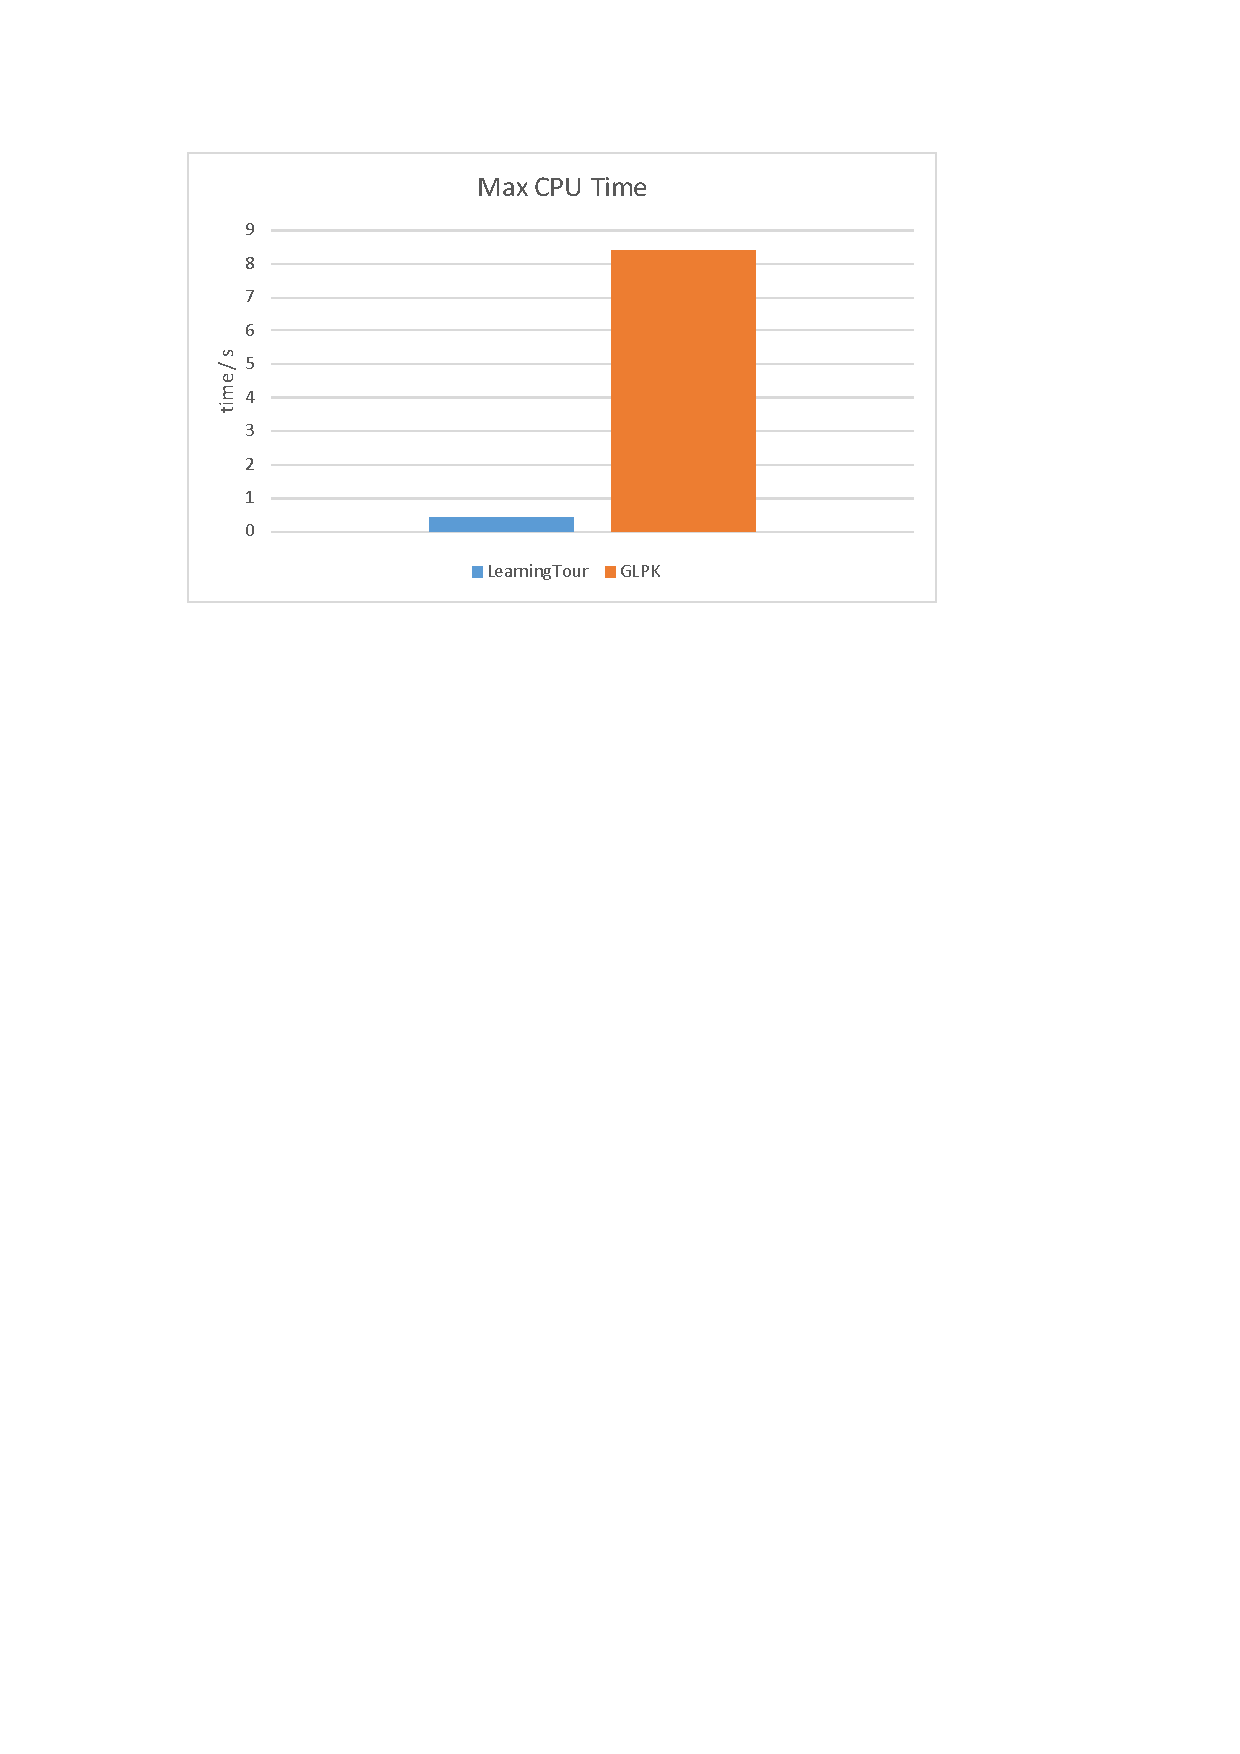
\includegraphics[width=0.48\textwidth]{MTO.pdf}}
	\caption{Max CPU Time of different solutions on two datasets}
	\label{fig:4}
\end{figure}
\section{Conclusions}
\quad\, In this article, we propose the LearningTour, a novel approach utilizing a encoder-decoder model for tour recommendation and taking other users' historical travel experience into account. This approach encodes users' interest to a context vector and decodes the vector to the recommended route. The result of our experiments based real datasets shows that our approach can effectively and rapidly recommends an appealing route, whereas we found our model can not recommend routes for a new city different from the city of the training data and also took a quite long time for the offline training. We also found that our model lacks the ability to recommend multiple-tour for one user. In the future, we will investigate the multi-cities training task and the similarities between cites to explant our model for other cities and try to ameliorate our model to support recommending routes during several days.
%
% the environments 'definition', 'lemma', 'proposition', 'corollary',
% 'remark', and 'example' are defined in the LLNCS documentclass as well.
%

%
% ---- Bibliography ----
%
% BibTeX users should specify bibliography style 'splncs04'.
% References will then be sorted and formatted in the correct style.
%
% \bibliographystyle{splncs04}
% \bibliography{mybibliography}
%
%\begin{thebibliography}{8}
%\bibitem{ref_article1}
%Author, F.: Article title. Journal \textbf{2}(5), 99--110 (2016)
%
%\bibitem{ref_article2}
%
%\bibitem{ref_lncs1}
%Author, F., Author, S.: Title of a proceedings paper. In: Editor,
%F., Editor, S. (eds.) CONFERENCE 2016, LNCS, vol. 9999, pp. 1--13.
%Springer, Heidelberg (2016). \doi{10.10007/1234567890}
%
%\bibitem{ref_book1}
%Author, F., Author, S., Author, T.: Book title. 2nd edn. Publisher,
%Location (1999)
%
%\bibitem{ref_proc1}
%Author, A.-B.: Contribution title. In: 9th International Proceedings
%on Proceedings, pp. 1--2. Publisher, Location (2010)
%
%\bibitem{ref_proc3}
%Takeshi Kurashima, Tomoharu Iwata, Go Irie, Ko Fujimura: Travel route recommendation using geotags in photo sharing sites. In: Proceedings of the 19th ACM international conference on Information and knowledge management (CIKM '10). ACM, New York, NY, USA, 579-588
%
%\bibitem{ref_url1}
%LNCS Homepage, \url{http://www.springer.com/lncs}. Last accessed 4
%Oct 2017
%\end{thebibliography}
\bibliographystyle{amsplain}
\bibliography{cite}
\end{document}
